\chapter{Results}

The predictions of the previous sections are tested on \emph{trans}-polyacetylene. Therefore the convergence is checked first. Since \emph{trans}-polyacetylene\footnote{In the following always \emph{trans}-polyacetylene is meant when only polyacetylene is said.} has an alternation of single and double bonds between the carbon atoms, a unit cell containing two CH-groups with periodic boundary conditions in one dimension is used (see \cref{image_scheme_polyacetylene_unit_cell}). 

\section{Convergence Testing of Polyacetylene}
\begin{figure}[]
	\centering
	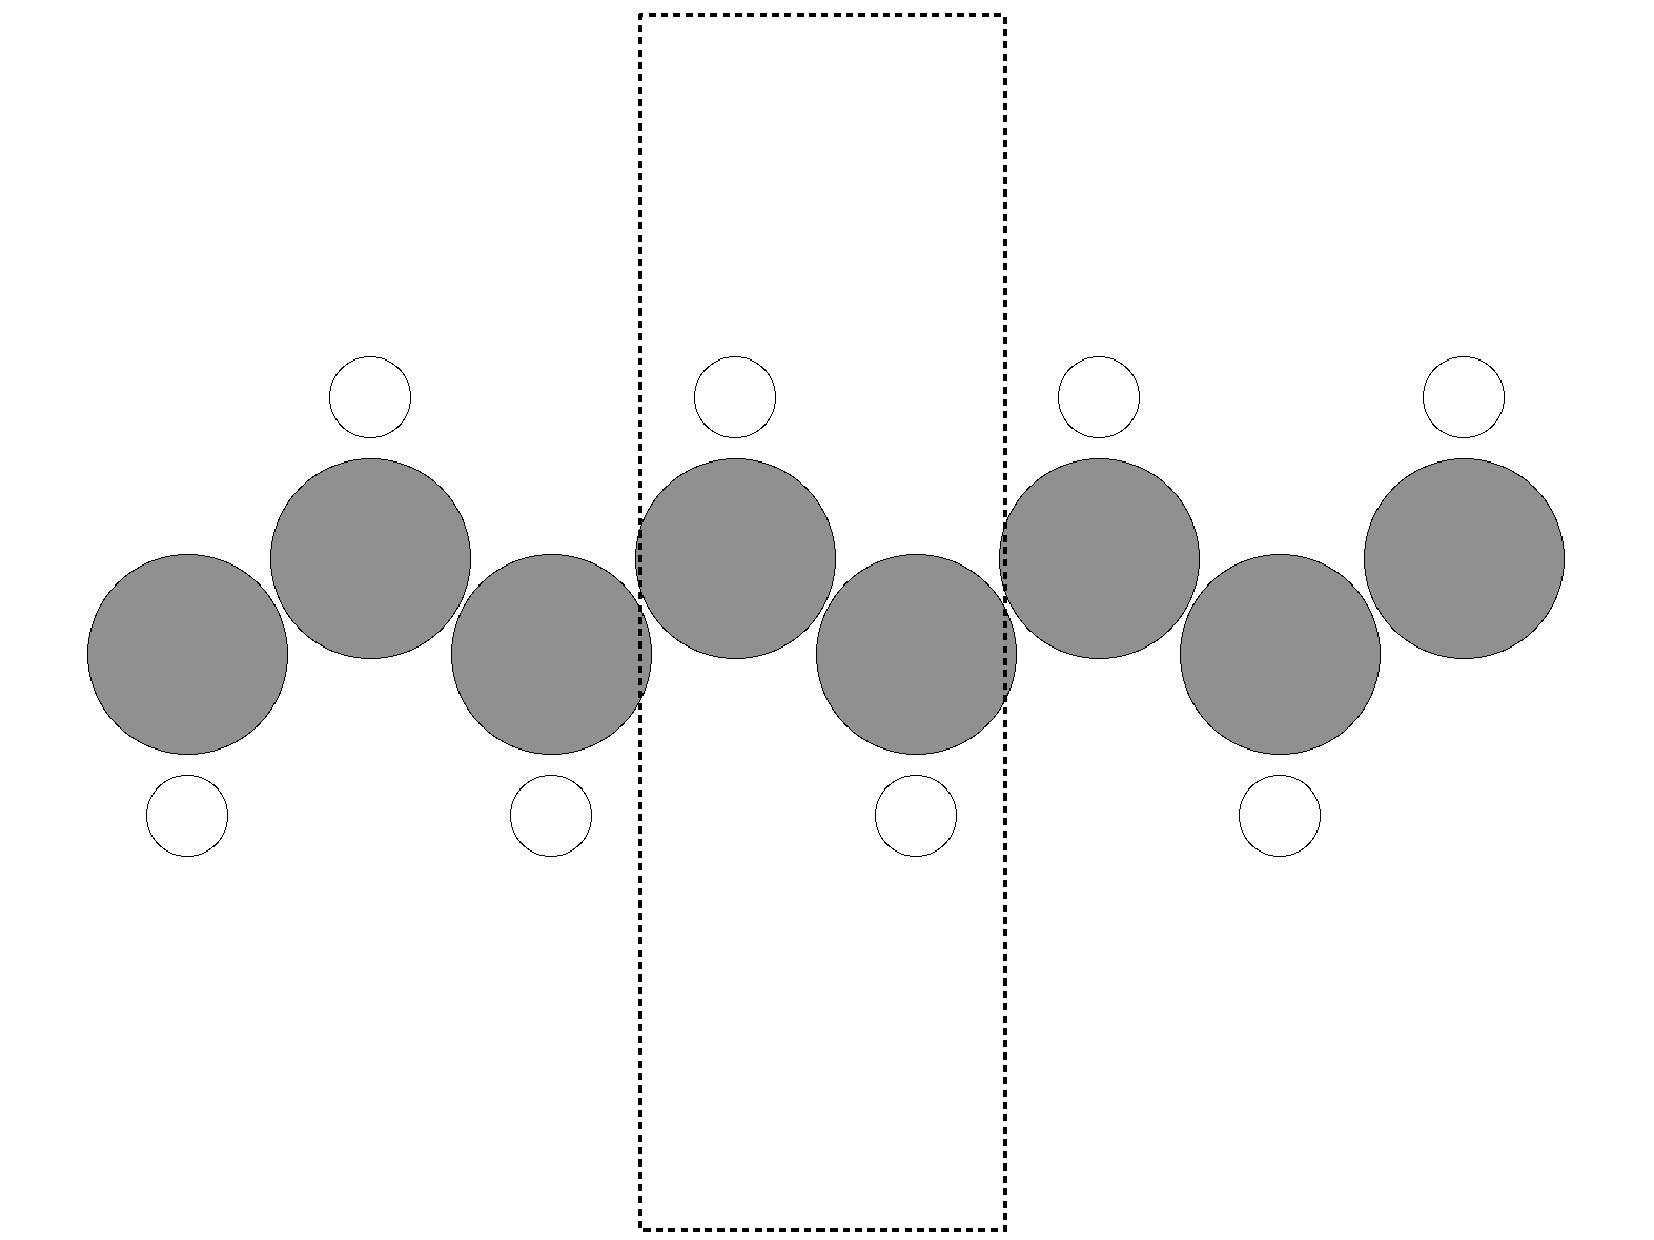
\includegraphics[width = .5\textwidth]{Images/polyacetylene/convergence/polyacetylene_nice_unit_cell}
	\caption{Scheme: Unit cell for \emph{trans}-polyacetylene with periodic boundary conditions in one dimension. The grey circles represent the carbon atoms, the white ones the hydrogen atoms.}
	\label{image_scheme_polyacetylene_unit_cell}
\end{figure}
To check the convergence in respect to a certain parameter, all other parameters are chosen in a way, that the energy is definitely converged in respect to them. This includes also a relaxation of the atom positions in each step.\\
First the convergence of the ground state energy in respect to the number of used $k$- points is tested, whereat automatic \textsc{Brillouin} zone sampling is used. It can be seen, that the energy is quite good converged for approximately 15 $k$-points (see \cref{image_poly_kpts_energy}), since a comparison of the energies for $15$ and $100$ $k$-points leads to a difference of only $\unit[0.014]{eV}$.\\
In \cref{image_poly_grid_energy} the ground state energy in respect to the grid spacing can be seen. Since the number of grid points grows with $\nicefrac{1}{h^3}$, it is very important to find a reasonable compromise between computing time and accuracy. Because our system isn't that big, a $h$ value of $\unit[0.1]{\AA}$ is used for further calculations.\\
The lowering of the ground state energy in respect to the maximum force for the relaxation process of the cores is in comparison with previous dependencies small (see \cref{image_poly_force_energy}). Therefore a maximum force of $\unitfrac[0.1]{eV}{\AA}$ should be appropriate.\\
Finally the convergence of the energy in respect to the unit cell width (not in the direction of the periodic boundary condition) is tested. As can be seen in \cref{image_poly_width_energy}, the ground state energy increases for small unit cell widths, what can be understood intuitively by comparison to the quantum mechanical 'particle in a box'. For a with of approximately $\unit[9]{\AA}$ a stable level is reached, what corresponds with a minimal distance between cores and cell surface of approximately $\unit[3]{\AA}$ (same for second direction of non periodic boundaries).\\
Convergence testing for other systems is done analogously and thus is added to the appendix.

\begin{figure}[]
	\centering
	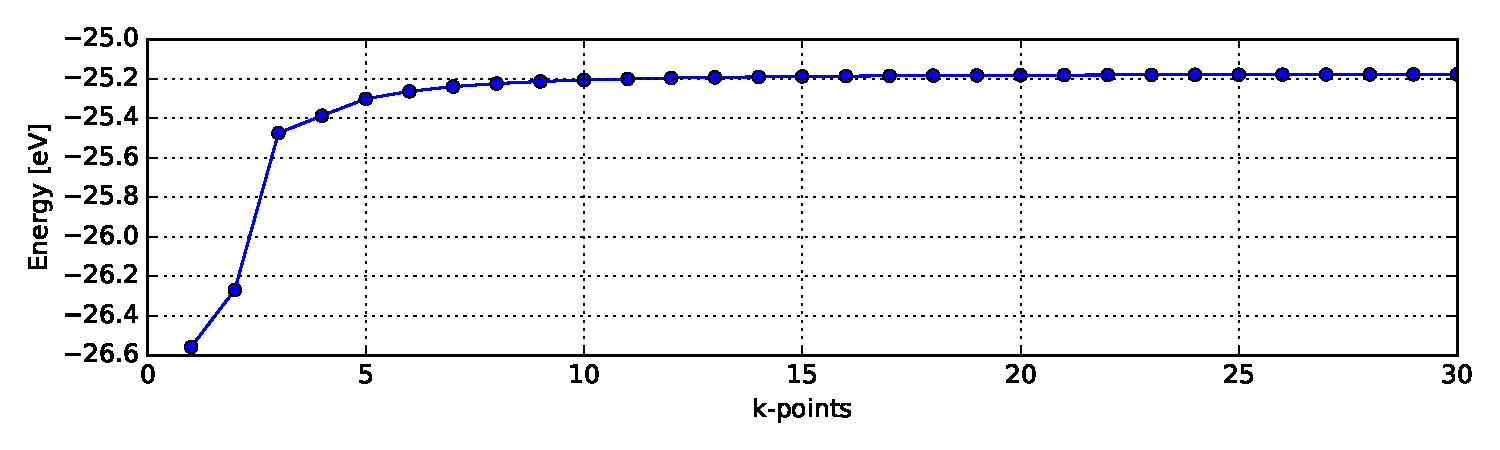
\includegraphics[width = 13cm]{Images/polyacetylene/convergence/kpts-energy}
	\caption{Ground state energy of relaxed polyacetylene in respect to the number of $k$-points}
	\label{image_poly_kpts_energy}
\end{figure}
\begin{figure}[]
	\centering
	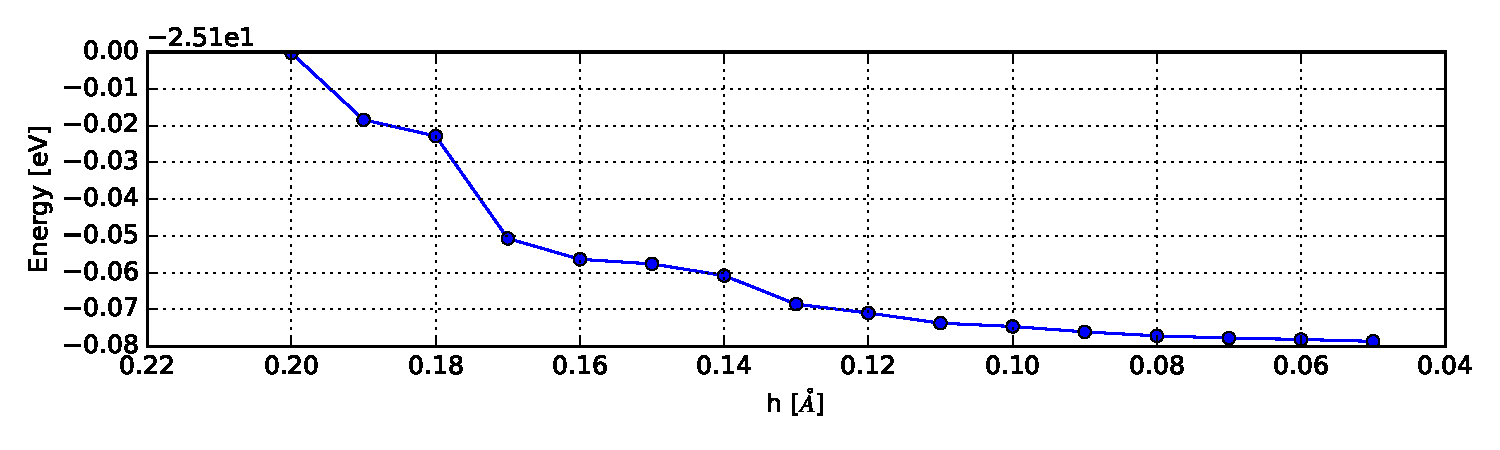
\includegraphics[width = 13cm]{Images/polyacetylene/convergence/gridspacing-energy}
	\caption{Ground state energy of relaxed polyacetylene in respect to the grid spacing}
	\label{image_poly_grid_energy}
\end{figure}
\begin{figure}[]
	\centering
	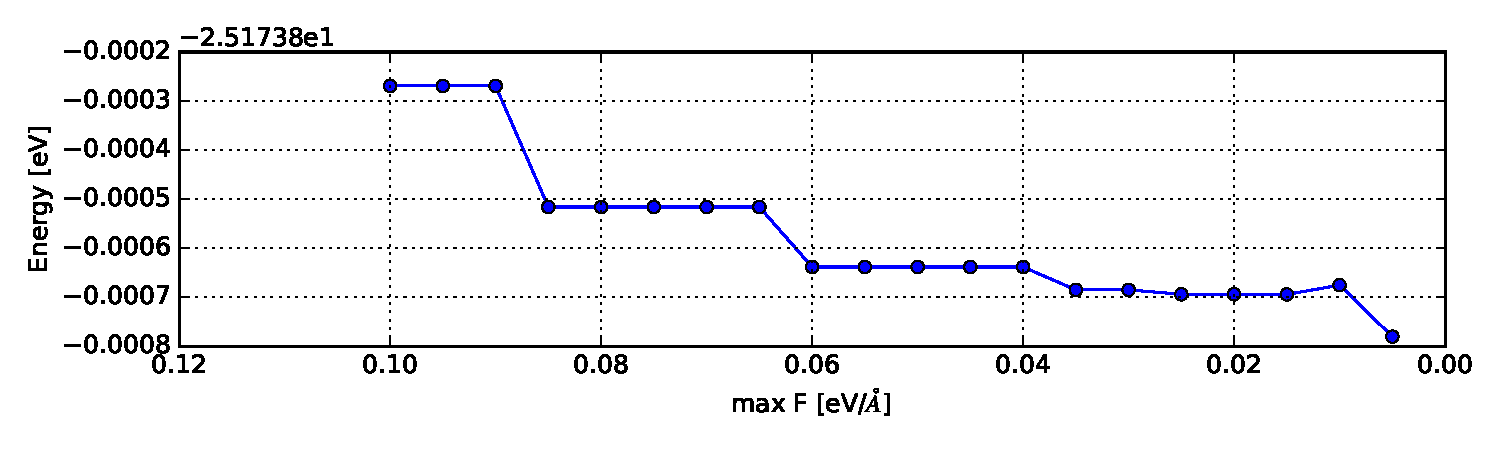
\includegraphics[width = 13cm]{Images/polyacetylene/convergence/forces-energy}
	\caption{Ground state energy of relaxed polyacetylene in respect to the maximum force, for which the relaxation process stops}
	\label{image_poly_force_energy}
\end{figure}
\begin{figure}[]
	\centering
	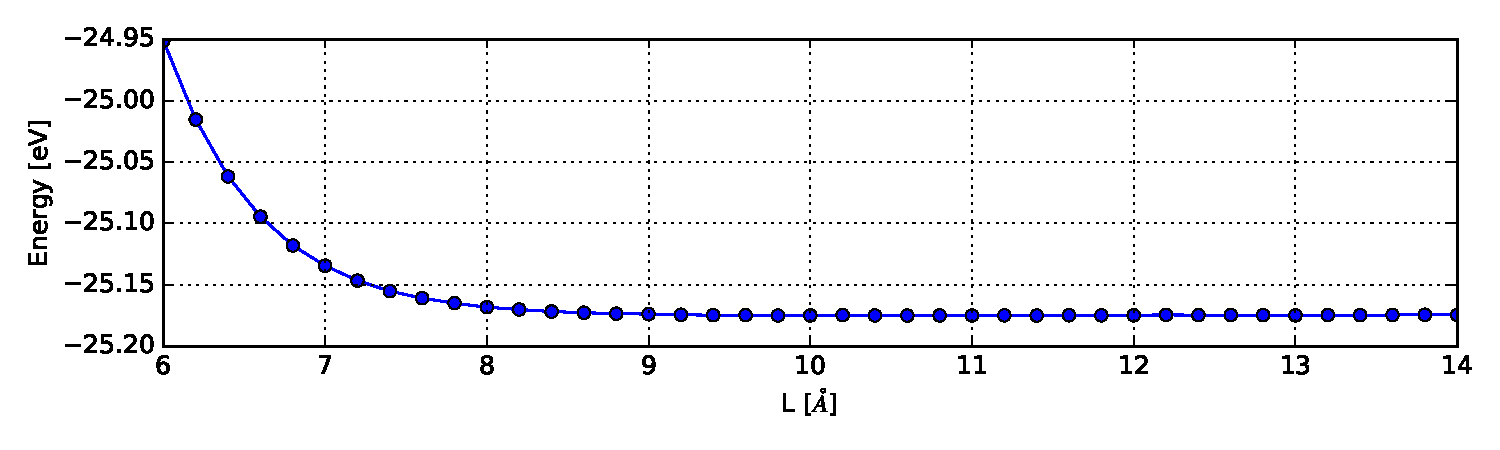
\includegraphics[width = 13cm]{Images/polyacetylene/convergence/unit_cell_width}
	\caption{Ground state energy of relaxed polyacetylene in respect to the width of the unit cell (not in direction of periodic boundary condition)}
	\label{image_poly_width_energy}
\end{figure}
\newpage


\section{Physical Quantities of Polyacetylene}
First, the bond length in direction of the periodic boundaries $a$ is calculated (see \cref{image_trans_polyacetylene}). This quantity corresponds with the half unit cell length (in the direction of periodic boundaries) and thus is calculated by minimizing the ground state energy in respect to the cell length (see \cref{image_poly_cell_len}). Through a quadratic fit a parameter of $a = \unit[1.23]{\AA}$ is obtained, what matches a literature value of $\unit[1.2]{\AA}$ (from \cite{PhysRevLett.42.1698}) perfectly.\\
\begin{figure}[!h]
	\centering
	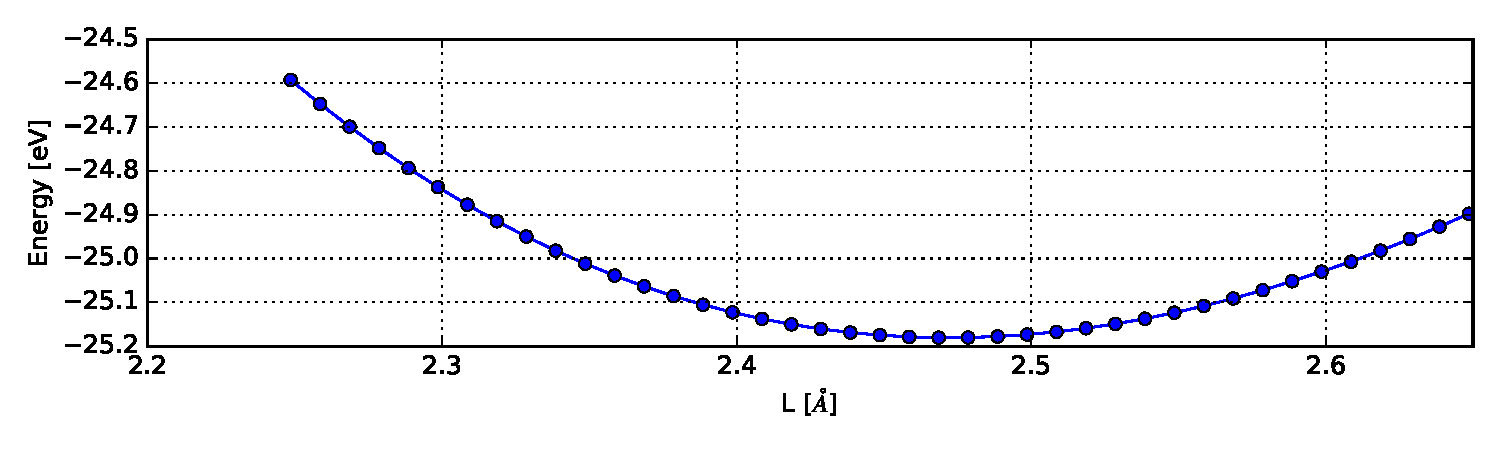
\includegraphics[width = 13cm]{Images/polyacetylene/convergence/unit_cell_length}
	\caption{Ground state energy of relaxed polyacetylene in respect to the length of the unit cell in direction of periodic boundaries}
	\label{image_poly_cell_len}
\end{figure}
\\
Second, the displacement $u$ of the carbon atoms is checked. Here, no distortion at all is obtained ($u < \unit[10^{-4}]{\AA}$) by using automatic $k$-point sampling, which doesn't include a $k$-point directly at the edge of the \textsc{Brillouin} zone. If the $k$-points are chosen manually in the way that a $k$-point at the edge of the \textsc{Brillouin} zone is included a bigger displacement of approximately $u = \unit[5\cdot10^{-3}]{\AA}$ is obtained (see \cref{image_k_point_sampling_assymetry}). In comparison to a literature value of $u = \unit[0.042]{\AA}$ (from \cite{PhysRevLett.42.1698, doi:10.1021/cr990357p}) it is still one order of magnitude to small, but it is known that PBE delocalizes electrons to much, which results in to small distortions and therefore in to small band gaps (see \cite{JIANG2009120,PhysRevB.84}).\\
\begin{figure}
	\centering
	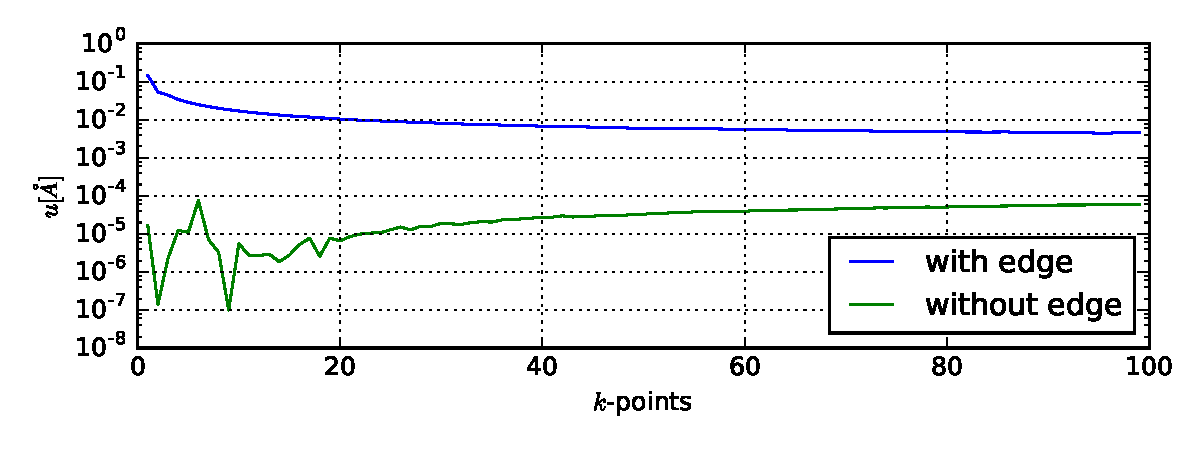
\includegraphics[width = 13cm]{Images/polyacetylene/convergence/polyacetylene_displacement}
	\caption{Displacement $u$ of the carbon atoms in respect to the number of $k$-points for automatic sampling (without $k$-point at the edge of the \textsc{Brillouin} zone) and manually placed $k$-points (with one $k$-point at the edge of the \textsc{Brillouin} zone).}
	\label{image_k_point_sampling_assymetry}
\end{figure}
In \cref{image_potential_with_asymmetry,image_potential_without_asymmetry} the ground state energies in respect to the asymmetry $\nicefrac{u}{u_0}$, whereat $u_0$ denotes the earlier obtained displacement, can be seen. For the case of $k$-points including the edge of the \textsc{Brillouin} zone (\cref{image_potential_with_asymmetry}), a twofold degeneracy of the ground state corresponding with the displacements $u = \pm u_0$ can be seen, which arises from the symmetry of the problem. In contradiction to this a non degenerate ground state, corresponding with no asymmetry, is obtained in the case of excluding the edge of the \textsc{Brillouin} zone (\cref{image_potential_without_asymmetry}).\\
\begin{figure}
	\centering
	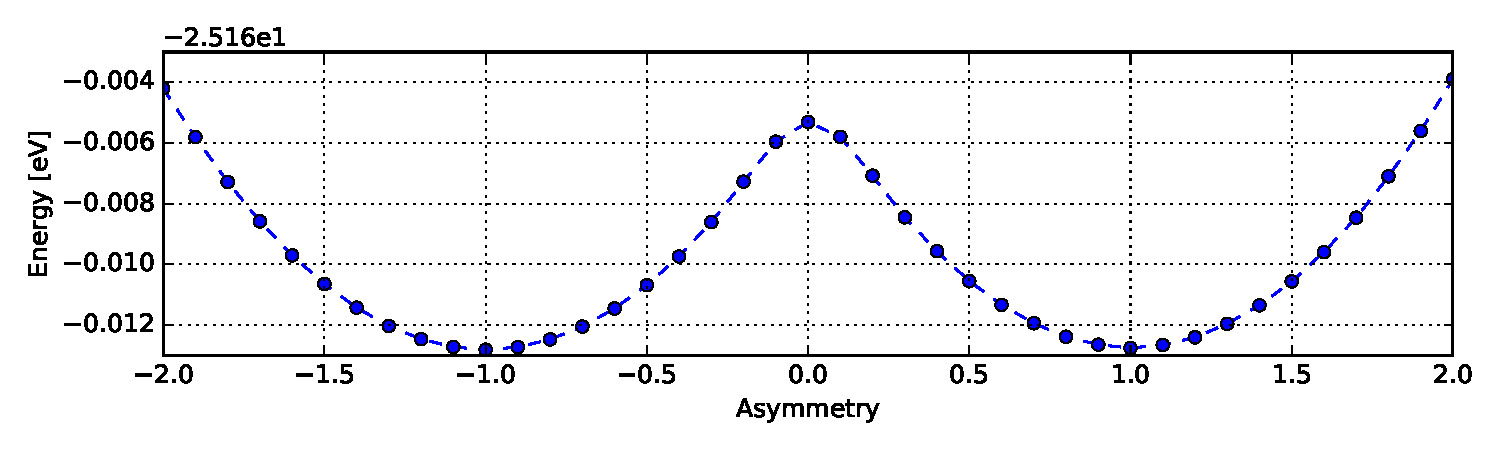
\includegraphics[width = 13cm]{Images/polyacetylene/convergence/Potential_with_asymmetry}
	\caption{Ground state energy for manually displaced atoms for calculations including a $k$-point at the edge of the \textsc{Brillouin} zone.}
	\label{image_potential_with_asymmetry}
\end{figure}
\begin{figure}[!p]
	\centering
	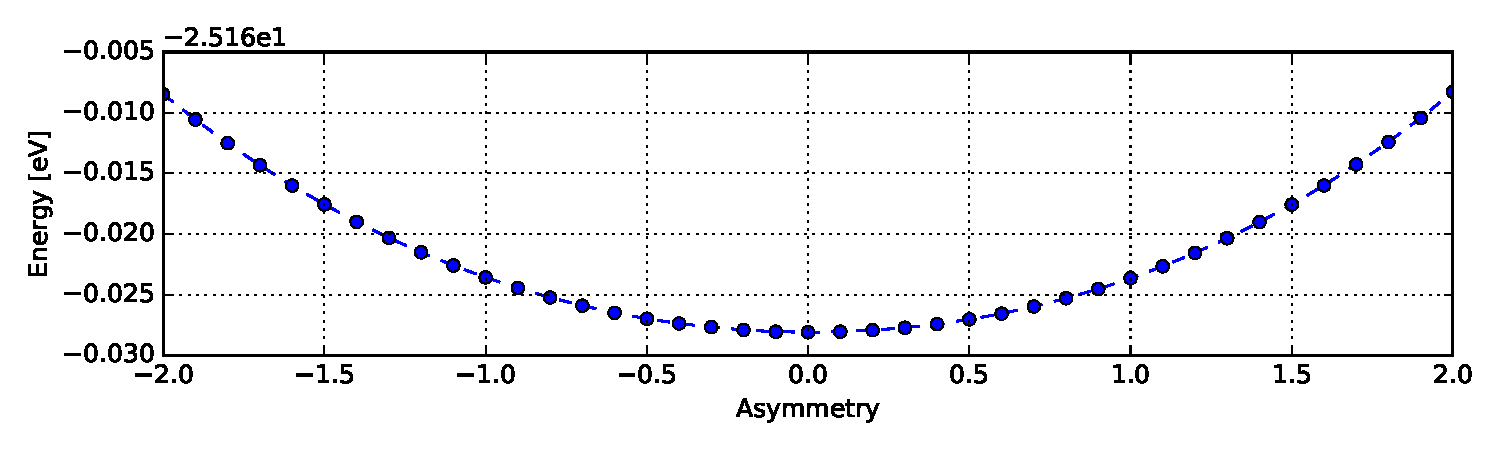
\includegraphics[width = 13cm]{Images/polyacetylene/convergence/Potential_without_asymmetry}
	\caption{Ground state energy for manually displaced atoms for calculations excluding a $k$-point at the edge of the \textsc{Brillouin} zone.}
	\label{image_potential_without_asymmetry}
\end{figure}
\begin{figure}[!p]
	\centering
	\begin{tikzpicture}[show background rectangle, scale = 1]
	\foreach \x in {0,...,7}{
		\draw[line width=2pt] (\x,0) .. controls (\x + 1, 2) and (\x - 1 , 2) .. cycle .. controls (\x + 1, -2) and (\x - 1 , -2) .. cycle;
	}
	\foreach \x in {0, 4}
	\foreach \y in {0, 1}
	\foreach \z in {-1, 1}
	\node at (\x + \y - \z + 1, \z) {\large +};
	\foreach \x in {0, 4}{
		\foreach \y in {0, 1}{
			\foreach \z in {-1, 1}{
				\node at (\x + \y - \z + 1, -\z) {\large -};
	}}}
	\draw[line width = 0.2] (-0.1, -1.8) -- +(-0.3, 0) -- +(-0.3 ,3.6) -- +(0,3.6);
	\draw[line width = 0.2] (1.1, -1.8) -- +(0.3, 0) -- +(0.3 ,3.6) -- +(0,3.6);
	\draw[line width = 0.2] (3.9, -1.8) -- +(-0.3, 0) -- +(-0.3 ,3.6) -- +(0,3.6);
	\draw[line width = 0.2] (7.1, -1.8) -- +(0.3, 0) -- +(0.3 ,3.6) -- +(0,3.6);
	\draw[dotted, line width = 1.5] (-0.6,0) -- (-1,0);
	\draw[dotted, line width = 1.5] (7.6,0) -- (8,0);
	\end{tikzpicture}
	\caption{Scheme: Sign of p-orbitals in a linear chain, that form an alternating $\pi$ bond. The phase difference of two adjacent unit cells, which contain two carbon atoms, is given by $\pi$, whereas the phase difference of two adjacent unit cells, each with four carbon cores, is given by zero.}
	\label{image_scheme_pi_bonds}
\end{figure}
\begin{figure}[!p]
	\centering
	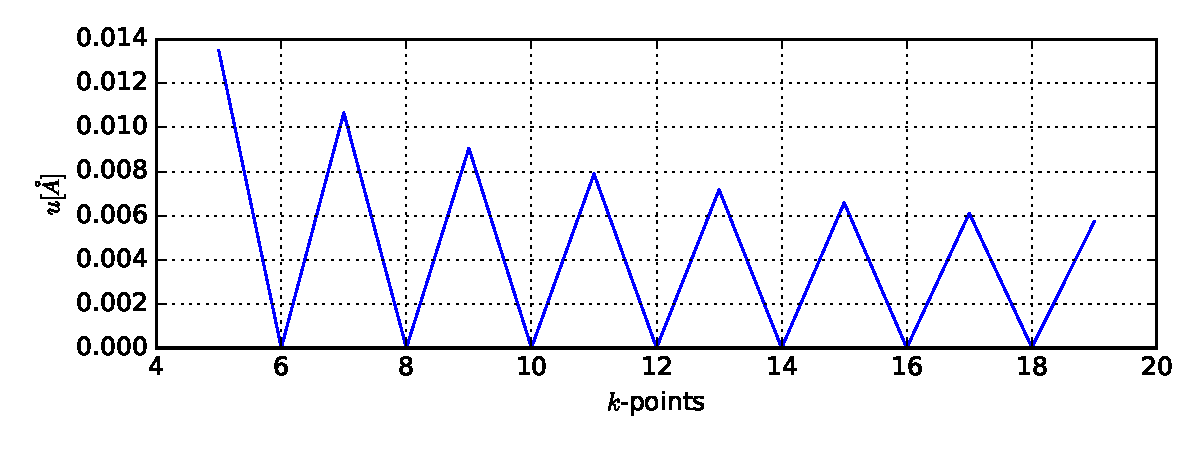
\includegraphics[width = 13cm]{Images/polyacetylene/convergence/displacement_double_cell_poly}
	\caption{Displacement $u$ of the carbon atoms in respect to the number of $k$-points for automatic sampling. The gamma point is automatically included for odd numbers of $k$-points, which leads to some asymmetry.}
	\label{image_disp_double_cell_poly}
\end{figure}
The importance of the $k$-point at the edge of the \textsc{Brillouin} zone can be understood by looking at the sign of the p-orbitals of carbon, which form an alternating $\pi$-bond (see \cref{image_scheme_pi_bonds}). 
\begin{figure}[!b]
	\centering
	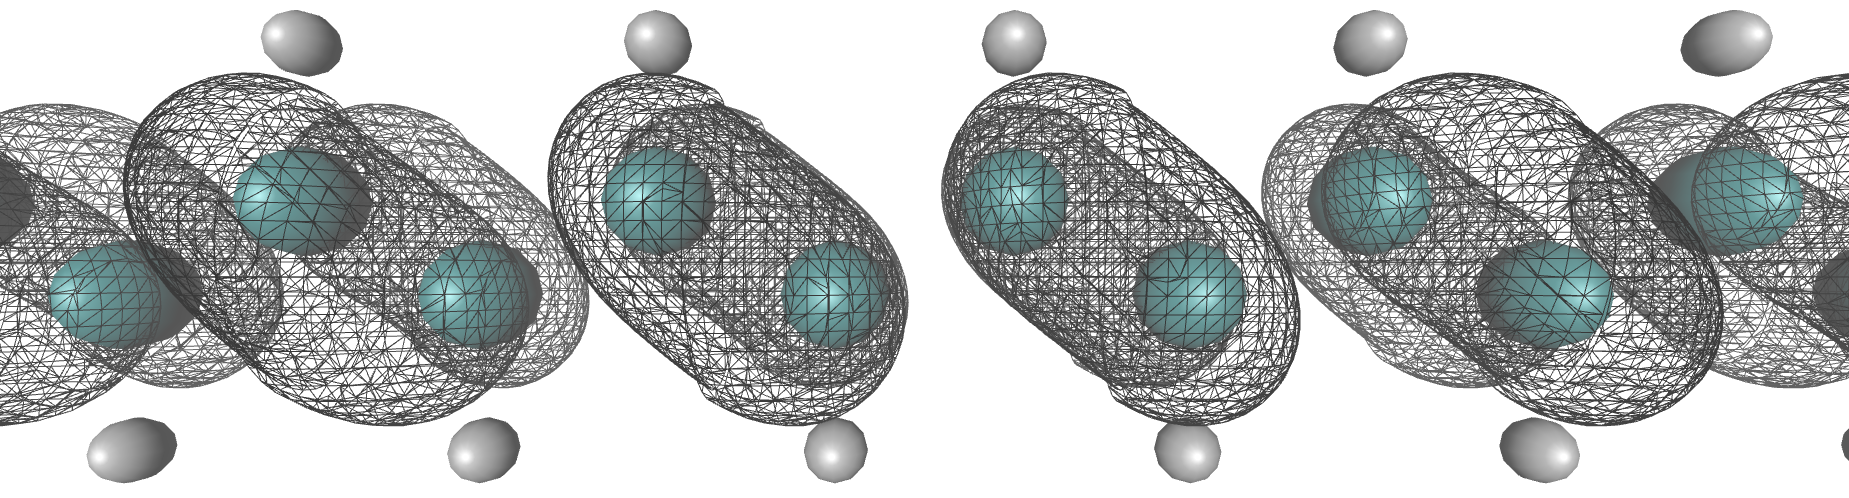
\includegraphics[width = 10cm]{Images/polyacetylene/wavefunctions/Homo}
	\caption{Isosurface for the HOMO-band state at the edge of the \textsc{Brillouin} zone.}
	\label{image_homo1}
\end{figure}
\begin{figure}[!b]
	\centering
	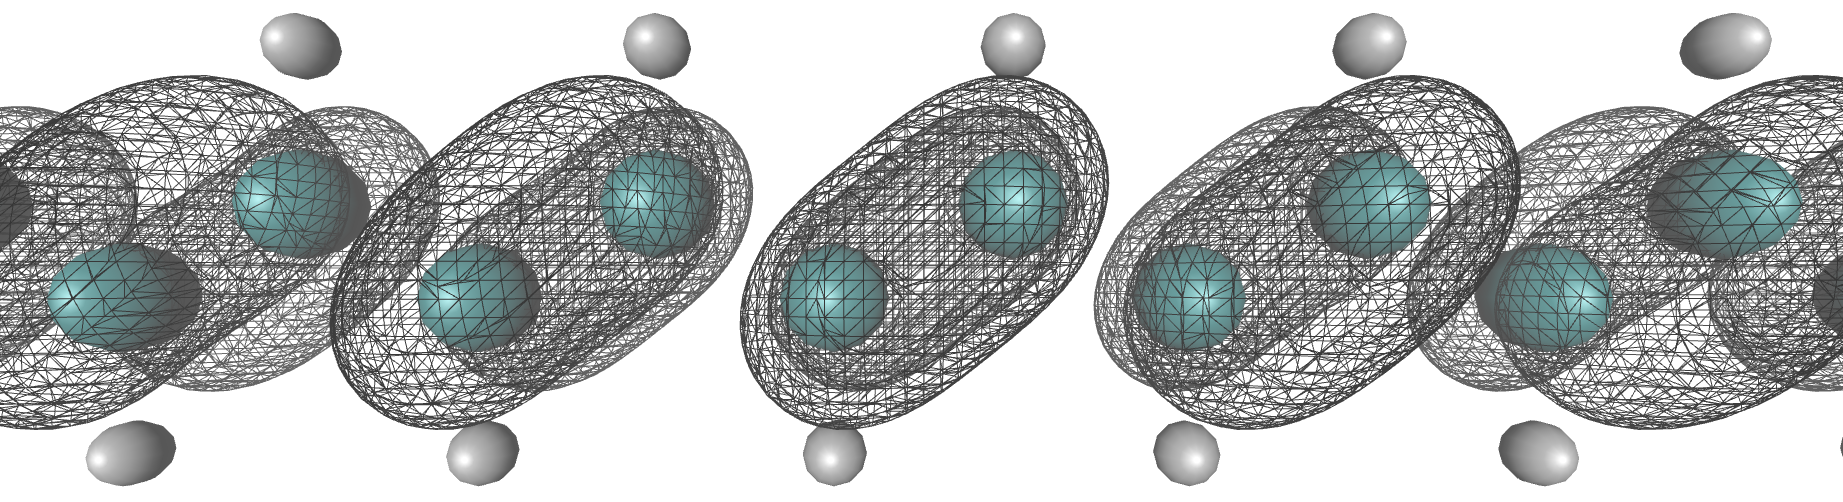
\includegraphics[width = 10cm]{Images/polyacetylene/wavefunctions/LUMO}
	\caption{Isosurface for the LUMO-band state at the edge of the \textsc{Brillouin} zone.}
	\label{image_lumo1}
\end{figure}
\begin{figure}[!b]
	\centering
	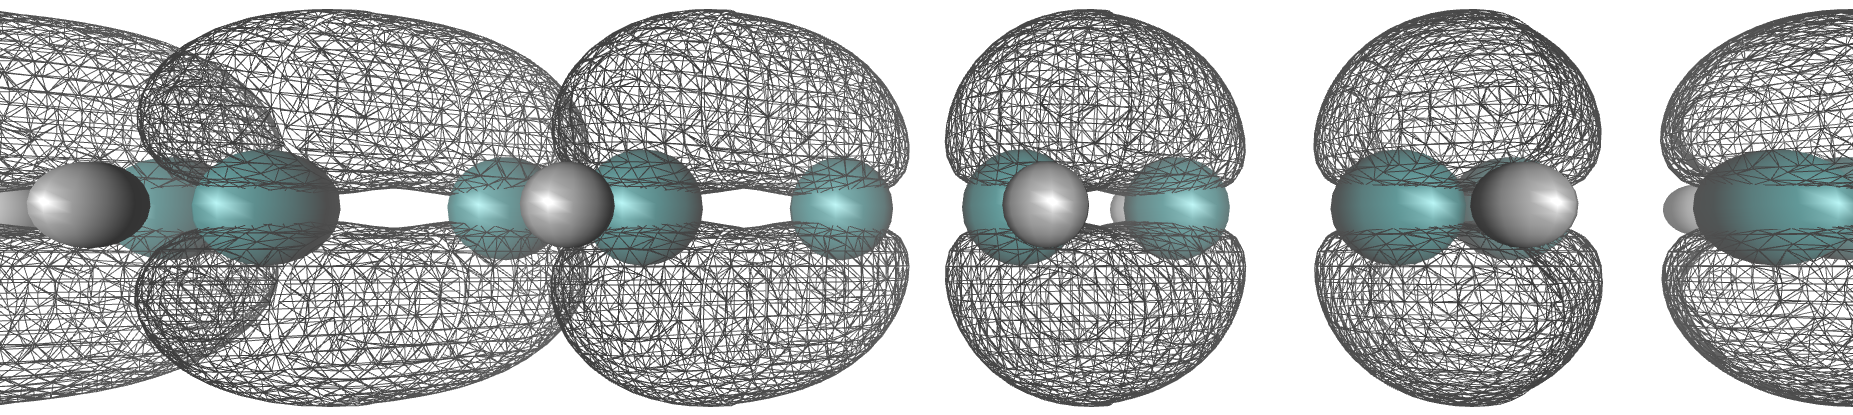
\includegraphics[width = 10cm]{Images/polyacetylene/wavefunctions/HOMO_Side_View}
	\caption{Side view of the isosurface for the HOMO-band state at the edge of the \textsc{Brillouin} zone. The typical 'out of plane' character of the $\pi$-bonds can be seen.}
	\label{image_homo1_side_view}
\end{figure}
Here a unit cell containing two carbon atoms needs a phase difference of $\pi$ between adjacent unit cells, what corresponds with a $k$-point at the edge of the \textsc{Brillouin} zone.\\
Consequently the gamma point is expected to be important for getting asymmetry in an unit cell containing four carbon atoms, since the phase difference of two such adjacent unit cells has to be $0$ to form alternating $\pi$-bonds. This is checked by simply using automatic $k$-point sampling, which includes the gamma point for an odd number of $k$-points automatically. As expected, an alternating behavior for the displacement in respect to the number of $k$-points can be seen in \cref{image_disp_double_cell_poly}.\\
Also the wave functions of the HOMO- and LUMO-band at the edge of the \textsc{Brillouin} zone show the expected forms (see \cref{image_homo1,image_lumo1,image_homo1_side_view}, where the turquoise balls represent the carbon atoms, the white ones the hydrogen atoms. All plots of isosurfaces are made with VMD \cite{HUMP96}). In particular this means, that the HOMO- and LUMO-band have basically the same form but form alternating $\pi$-bonds between opposite pairs of carbon. This would correspond with changing the sign of the p-orbitals of every second carbon atom in \cref{image_scheme_pi_bonds}, what can also be seen directly from the earlier derived eigenstates (see \cref{equation_conduction_eigenstate,equation_valence_eigenstate}). From the symmetry it can be concluded, that for $u=0$ this two states should have the same energy and therefore no band gap is expected.\\
\begin{figure}
	\centering
	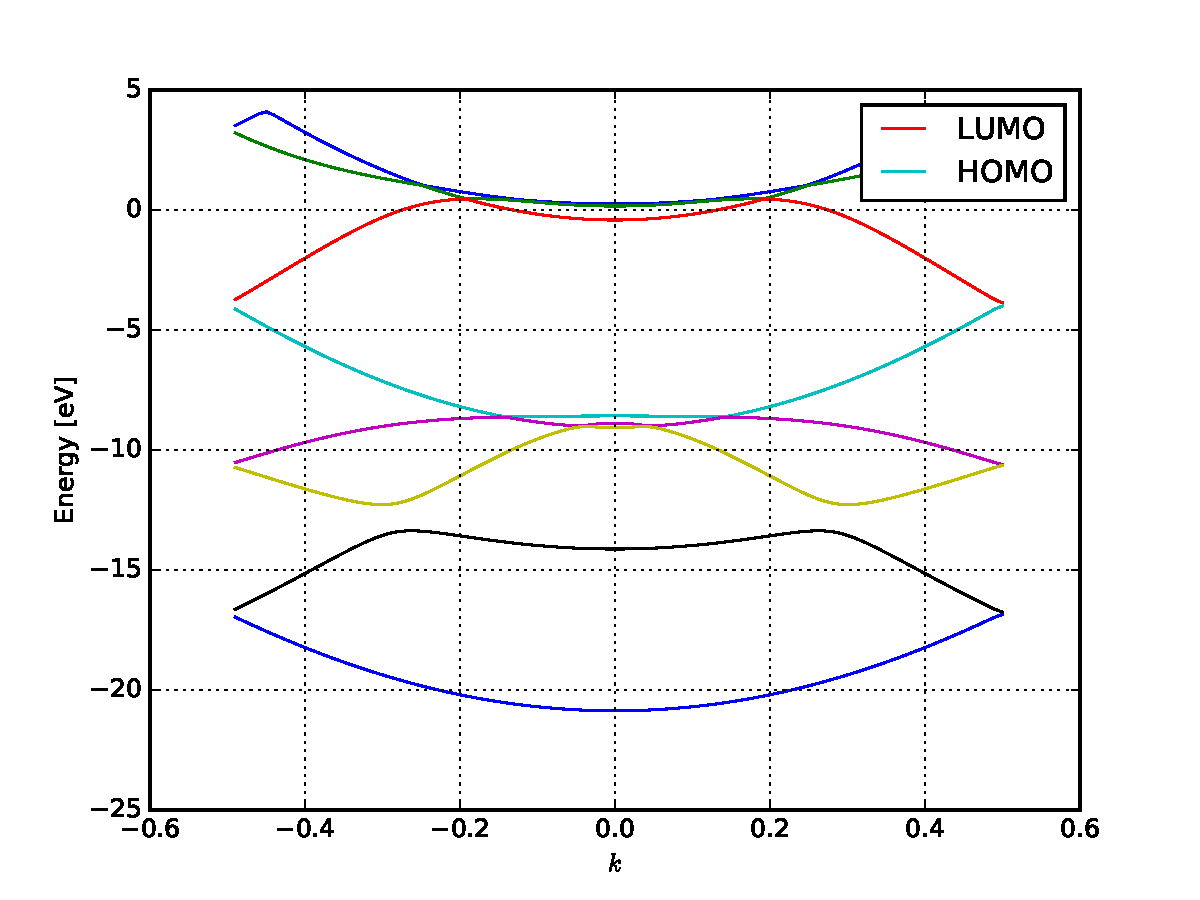
\includegraphics[width = 11cm]{Images/polyacetylene/bands/band_structure}
	\caption{Band structure of relaxed polyacetylene containing the five highest occupied bands and three unoccupied bands.}
	\label{image_band_structure_relaxed_polyacetylene}
\end{figure}
The band structure of the relaxed polyacetylene can be seen in \cref{image_band_structure_relaxed_polyacetylene}. Here and in the following plots of band structures the $k$-values are given in respect to the basis of the reciprocal lattice and thus a value of $k = \pm 0.5$ corresponds with a state at the edge at the \textsc{Brillouin} zone. As expected a very small band gap of approximately $E_\text{Gap} \approx \unit[0.137]{eV}$ between the HOMO- and LUMO-band can be seen. Again this mismatches a literature value of $E_\text{Gap} = \unit[1.4]{eV}$ (see \cite{PhysRevLett.42.1698}) by a complete order of magnitude. The form of the HOMO- and LUMO-band in the outer regions seems to be in good accordance with the predicted form (compare \cref{equation_energy_band}):
\begin{align}
E_k &= \pm \sqrt{\left(2t_0\cos(ka)\right)^2+\left(2\delta\sin(ka)\right)^2}
\label{equation_explicit_energy_band}
\end{align} In the central region some interaction between the bands occurs, which leads to the well known effect of \emph{avoided crossings} (see \cite{ashcroft}). This effect can also be seen by looking at the wave functions of the third and the HOMO-band at the $\Gamma$-point (see \cref{image_homo_mid_k,image_homo_mid_k_side_view,image_third_band,image_third_band_side_view}), which shows that for the $\Gamma$-point the third band and not the HOMO-band corresponds with the p-orbitals. Further it can be seen, that the state of the third band at the $\Gamma$-point drawn in the schematic way of \cref{image_scheme_pi_bonds} would have the same sign for all p-orbitals in the upper row and the other sign for all states in the lower row (see \cref{image_scheme_p_orbitals_gamma_point}).\\
\begin{figure}
	\centering
	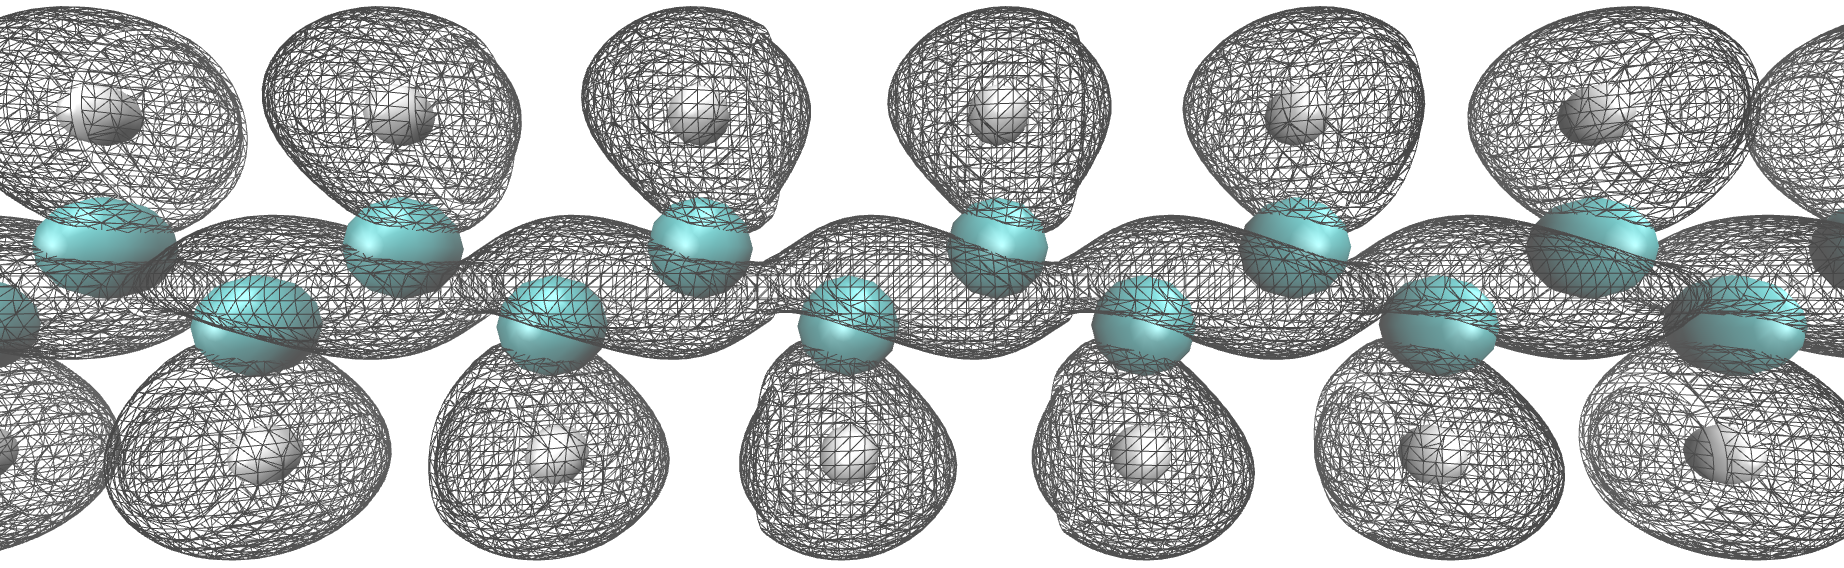
\includegraphics[width = 12cm]{Images/polyacetylene/wavefunctions/Homo_mid_k}
	\caption{Isosurface for the HOMO-band state at the $\Gamma$-point.}
	\label{image_homo_mid_k}
\end{figure}
\begin{figure}
	\centering
	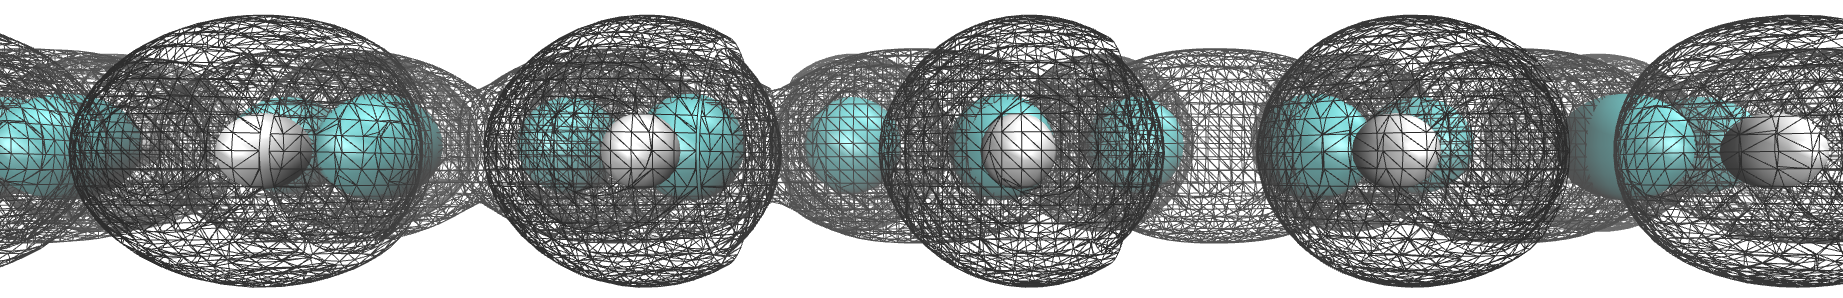
\includegraphics[width = 12cm]{Images/polyacetylene/wavefunctions/Homo_mid_k_Side_View}
	\caption{Side view of the isosurface for the HOMO-band state at the $\Gamma$-point without an 'out of plane' character.}
	\label{image_homo_mid_k_side_view}
\end{figure}
\begin{figure}
	\centering
	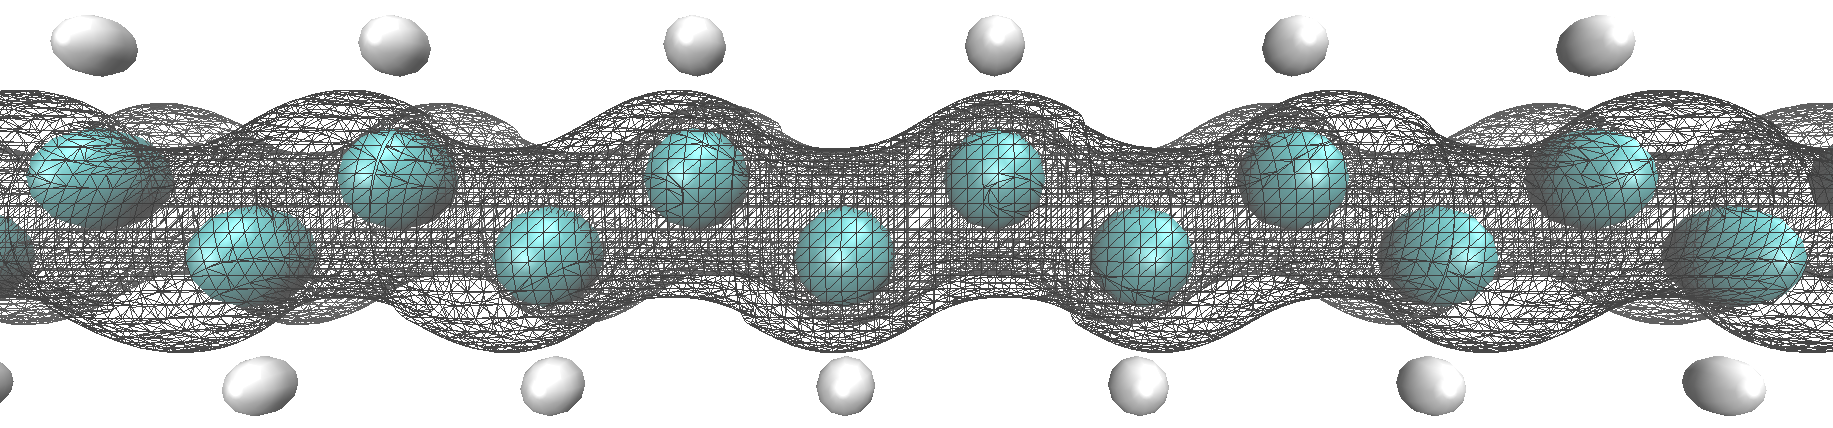
\includegraphics[width = 12cm]{Images/polyacetylene/wavefunctions/Mid_band_2}
	\caption{Isosurface of the third band at the $\Gamma$-point.}
	\label{image_third_band}
\end{figure}
\begin{figure}
	\centering
	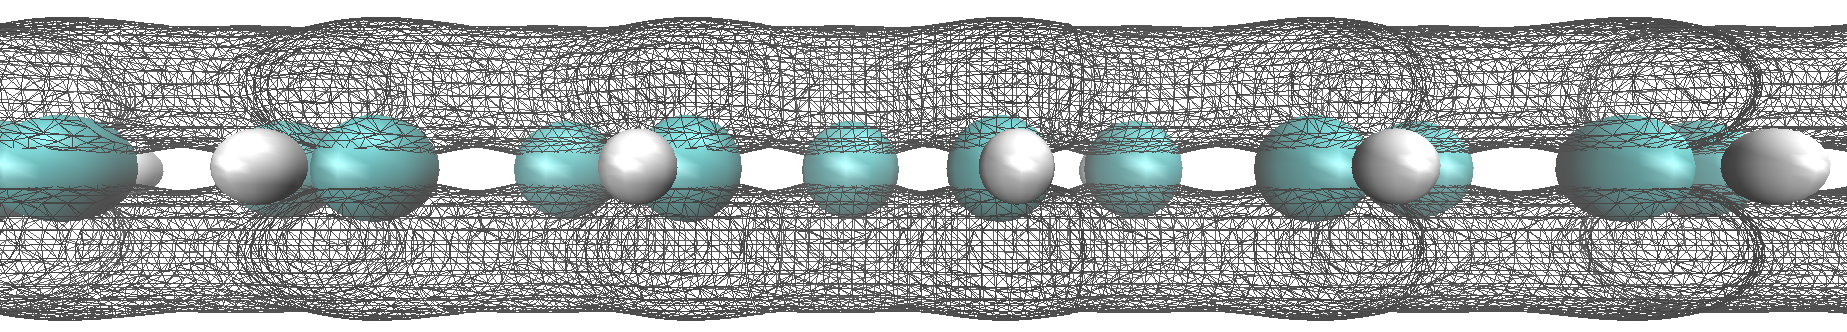
\includegraphics[width = 12cm]{Images/polyacetylene/wavefunctions/Mid_band_2_Side_View}
	\caption{Side view of the third band at the $\Gamma$-point, showing an 'out of plane' character.}
	\label{image_third_band_side_view}
\end{figure}
\begin{figure}
	\centering
	\begin{tikzpicture}[show background rectangle, scale = 1]
	\foreach \x in {0,...,7}{
		\draw[line width=1pt] (\x,0) .. controls (\x + 1, 2) and (\x - 1 , 2) .. cycle .. controls (\x + 1, -2) and (\x - 1 , -2) .. cycle;
	}
	\foreach \x in {0,...,7}{
		\foreach \y/\s in {-1/+, 1/-}{
			\node at (\x, \y) {\huge \s};}}
	\draw[dotted, line width = 1.5] (-0.6,0) -- (-1,0);
	\draw[dotted, line width = 1.5] (7.6,0) -- (8,0);
	\end{tikzpicture}
	\caption{Scheme: Sign of p-orbitals of the valence state at the $\Gamma$-point}
	\label{image_scheme_p_orbitals_gamma_point}
\end{figure}
To get the hopping parameter $t_0$ a fit with the form of \cref{equation_explicit_energy_band} is done to a continuous combination of the third, forth and fifth band (see \cref{image_band_fit_t0}), since band interactions aren't treated in this simple model. Thus a hopping parameter of $\unit[2.62]{eV}$ is obtained, what matches a literature value of approximately $\unit[2.5]{eV}$ (see \cite{PhysRevLett.42.1698}) very well.\\
To calculate the phonon coupling constant the following relation is used:
\begin{align}
	\alpha &= \frac{1}{8} \frac{\partial E_\text{Gap}}{\partial u}
\end{align}
Thus the band gap is calculated for different displacements $u$ and a linear fit is applied to this data (see \cref{image_alpha_fit}), whereat the phonon coupling constant is calculated from the slope. In this way a value of $\alpha = \unitfrac[3.95]{eV}{\AA}$ is obtained, which again matches a literature value of $\alpha = \unitfrac[4.1]{eV}{\AA}$ very well.\\
Finally the band gap for a manually displacement in accordance to the literature value of $u = \unit[0.042]{\AA}$ (from \cite{PhysRevLett.42.1698, doi:10.1021/cr990357p}) is calculated (see \cref{image_manually_displaced_poly_bandstructure}). This yields a band gap of $E = \unit[1.27]{eV}$, what is quite good in comparison with a literature value of $E_\text{Gap} = \unit[1.4]{eV}$ (see \cite{PhysRevLett.42.1698}).\\
A short summary of the results is given in \cref{table_summary_polyacetylene}.\\
\begin{figure}
	\centering
	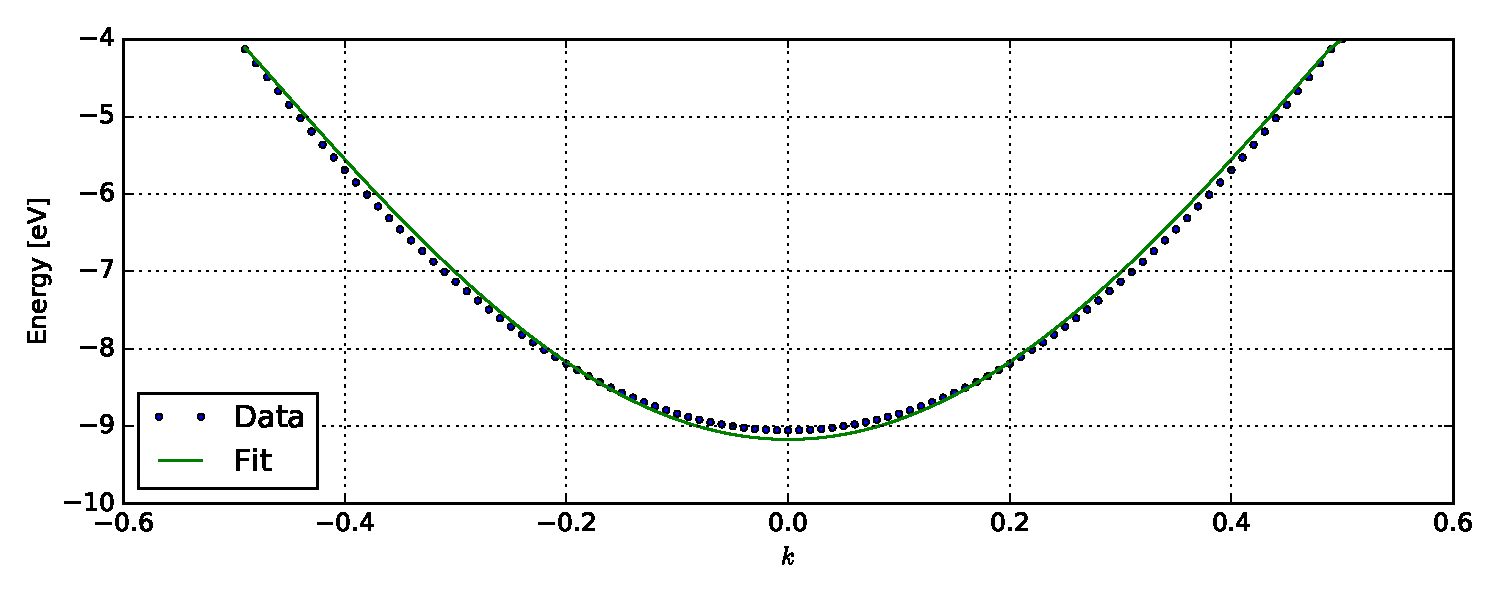
\includegraphics[width = 13cm]{Images/polyacetylene/bands/band_fit}
	\caption{Fit of the derived band form to a continuous combination of the third, forth and fifth band.}
	\label{image_band_fit_t0}
\end{figure}
\begin{figure}
	\centering
	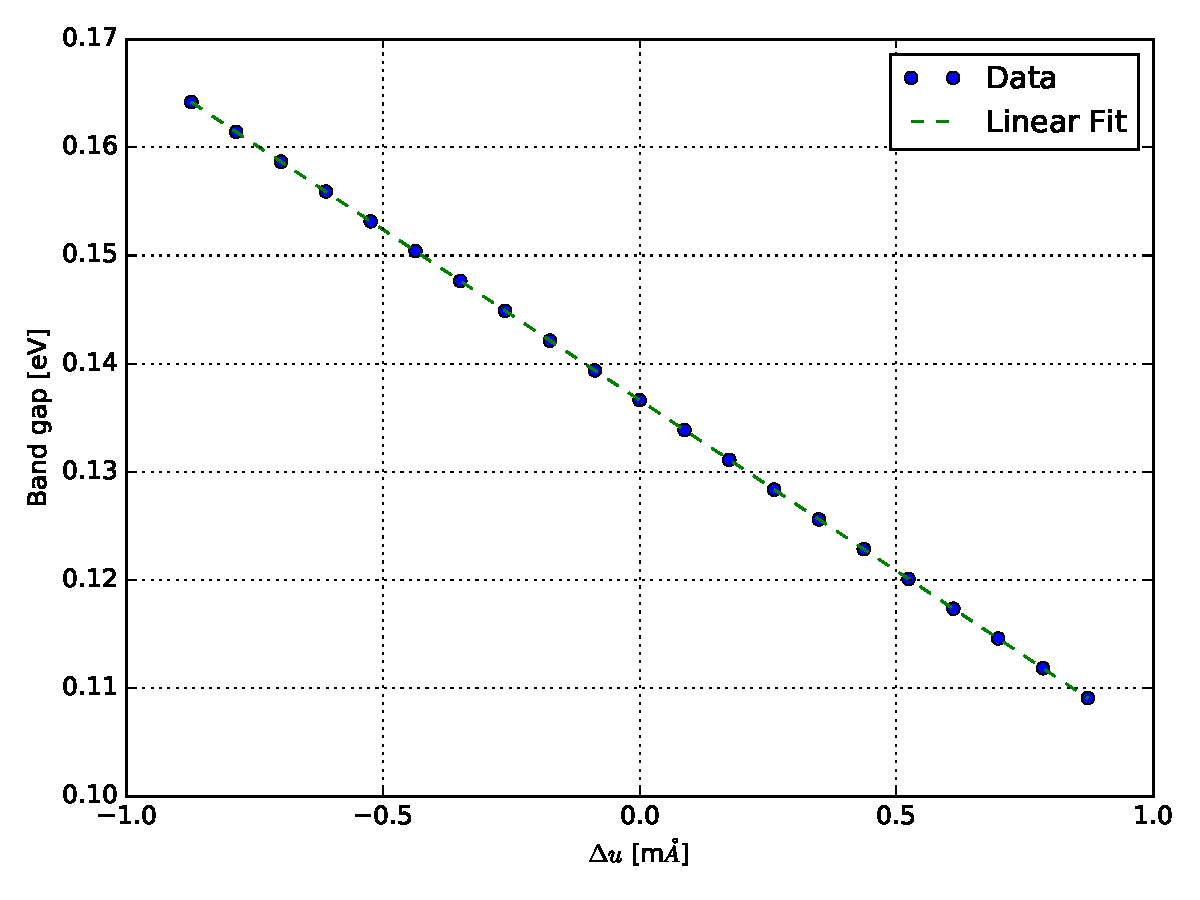
\includegraphics[width = 13cm]{Images/polyacetylene/bands/alpha}
	\caption{Band gap for manually displacements $u$ with a linear fit.}
	\label{image_alpha_fit}
\end{figure}
\begin{figure}
	\centering
	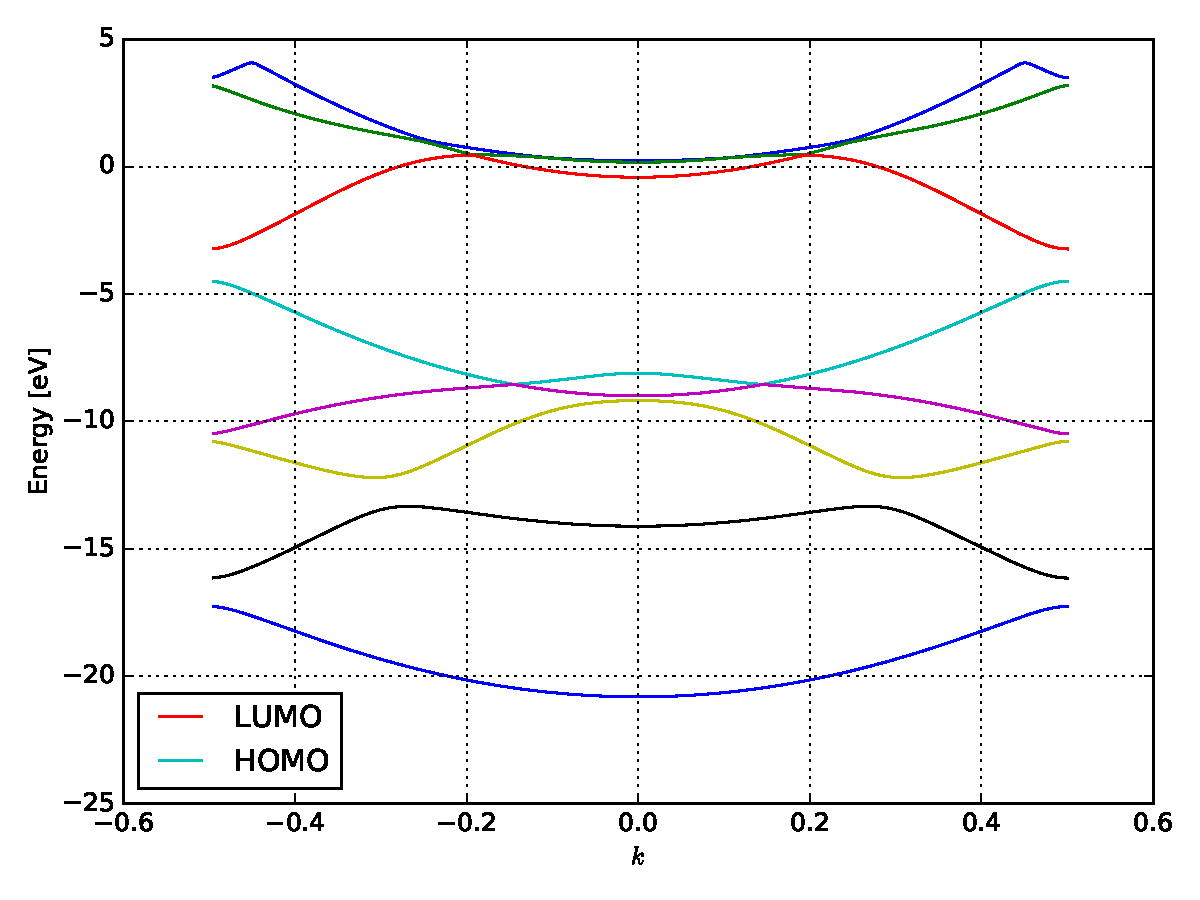
\includegraphics[width = 11cm]{Images/polyacetylene/bands/bandstructure_manually_displaced}
	\caption{Band structure of manually displaced polyacetylene.}
	\label{image_manually_displaced_poly_bandstructure}
\end{figure}
\begin{table}[]
	\centering
	\begin{tabular}{l|c|c}
	Quantety & Calculated Value & Literature Value (\cite{PhysRevLett.42.1698, doi:10.1021/cr990357p})\\
	\hline \hline
	&&\\[-.3cm]
	Bond length \hfill$a [\unit{\AA}]$ & $1.23$ & $1.2$\\ \hline&&\\[-.3cm]
	Displacement \hfill$u [\unit{\AA}]$& $0 - 5\cdot10^{-3}$ & $0.042$\\ \hline&&\\[-.3cm]
	Energy gap (manually displaced)\hfill$E_\text{Gap} [\unit{eV}]$ & $0.137\quad(1.27)$ & $1.4$\\ \hline &&\\[-.3cm]
	Hopping parameter \hfill$t_0 [\unit{eV}]$ & $2.62$ & $2.5$ \\ \hline&&\\[-.3cm]
	Phonon coupling constant \hspace*{2cm}$\alpha [\unitfrac{eV}{\AA}]$& $3.95$ & $4.1$
	\end{tabular}
	\caption{Summary of the results for polyacetylene.}
	\label{table_summary_polyacetylene}
\end{table}


\section{Constraint Density Functional Theory}
\label{section_constraint_density_functonal_theory}
In this section the influences of charging different regions using cDFT is studied and two alternative methods of calculating the hopping parameter $t_0$ are tested. First this is done for a system as simple as possible, namely a chain of equidistant hydrogen atoms.
\subsection{Chain of Hydrogen Atoms}
Even if there's no distortion, a unit cell with two hydrogen atoms is needed, because later the application of the external potential and the consequential charge displacement will break the symmetry. First, the unit cell length for the lowest ground state energy is determined to $L = \unit[2.0]{\AA}$ (see \cref{image_hydrogen_unit_cell_length}).
\begin{figure}
	\centering
	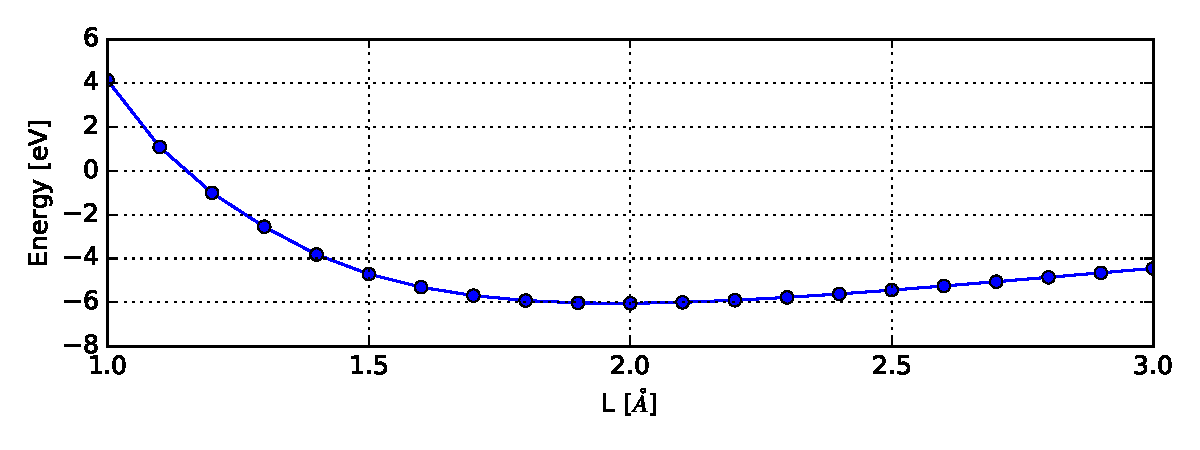
\includegraphics[width = 13cm]{Images/Hydrogen/convergence/hydrogen_length}
	\caption{Ground state energy of a unit cell containing two equidistant hydrogen atoms in respect to the unit cell length in direction of the periodic boundaries.}
	\label{image_hydrogen_unit_cell_length}
\end{figure}
\begin{figure}
	\centering
	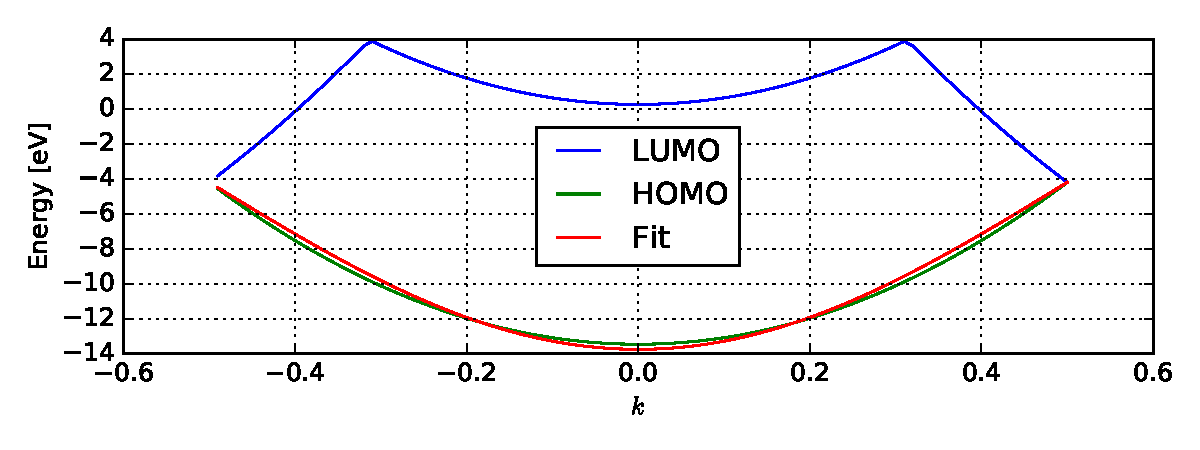
\includegraphics[width = 13cm]{Images/Hydrogen/bands/hydrogen_band_structure}
	\caption{Band structure of a hydrogen chain with a fit to its HOMO-band.}
	\label{image_hydrogen_band_structure}
\end{figure}
As can be seen in \cref{image_hydrogen_band_structure} the HOMO-band is in good accordance with the expected form\footnote{Since there's no distortion $\Delta_k = 0$ (compare \cref{equation_energy_band})} of:
\begin{align}
	E_k = -2t_0\cos(ka)
\end{align}
from which the hopping parameter $t_0 = \unit[4.8]{eV}$ is obtained. This value is used as reference later.\\
\begin{figure}
	\centering
	\begin{subfigure}{0.45\textwidth}
		\centering
		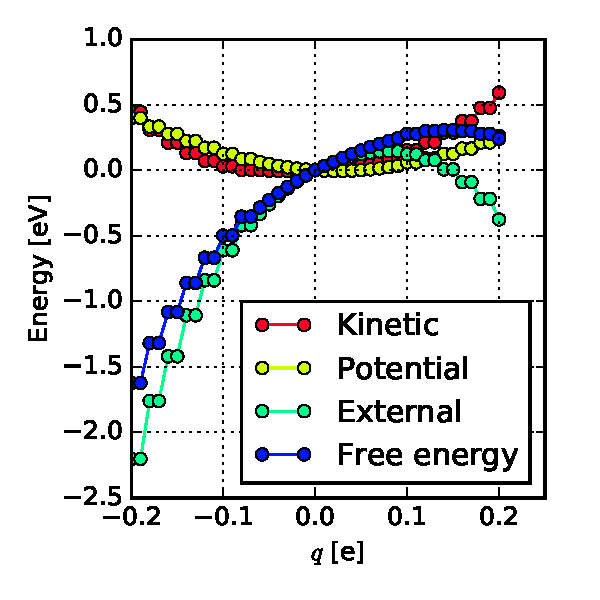
\includegraphics[width = \textwidth]{Images/Hydrogen/charging/energy_contributions_asymmetric}
		\caption{Initial}
		\label{image_contributions_initial}
	\end{subfigure}\hspace*{1cm}
	\begin{subfigure}{0.45\textwidth}
		\centering
		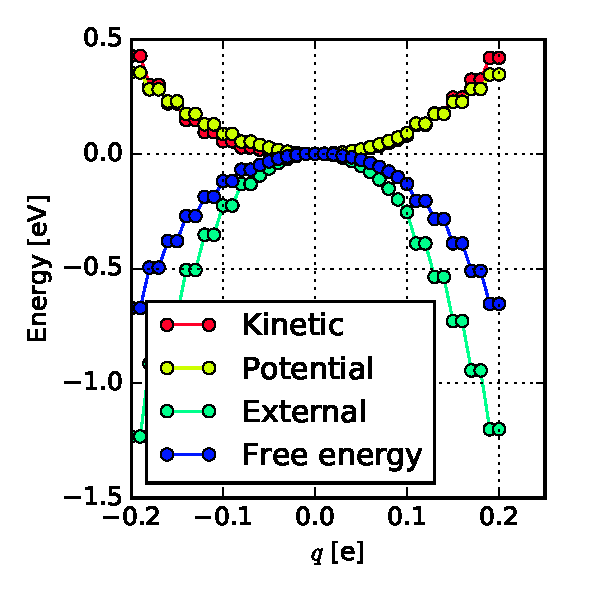
\includegraphics[width = \textwidth]{Images/Hydrogen/charging/energy_contributions_symmetric}
		\caption{Corrected}
		\label{image_contributions_corrected}
	\end{subfigure}
	\caption{Some energy contributions in respect to the displaced charge. The offsets are set to zero for $q=0$.}
\end{figure}
\begin{figure}
	\centering
	\begin{subfigure}{0.45\textwidth}
		\centering
		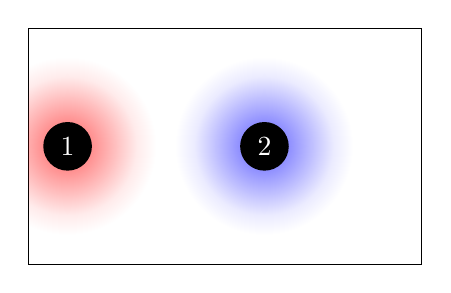
\begin{tikzpicture}[]
		\begin{scope}
		\clip [draw] (-.5, -1.5) rectangle (4.5, 1.5);
		\foreach \x/\color in {0/red, 2.5/blue}{
			\foreach \r in {0, 0.01, ..., 1}{
				\fill[opacity = \r * 0.02, fill = \color] (\x, 0) circle ({2.5 * (.5 - 0.5 * \r)});}}
		\foreach \x/\num in {0/1, 2.5/2}{
			\node[fill = black, shape = circle, text = white] at (\x, 0)	 {\num};}
		\end{scope}
		\end{tikzpicture}
		\caption{\textsc{Gaussian} curves cut at periodic boundary.\\}
	\end{subfigure}\hspace*{1cm}
	\begin{subfigure}{0.45\textwidth}
		\centering
		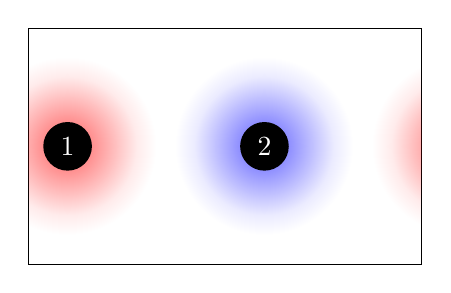
\begin{tikzpicture}
		\begin{scope}
		\clip [draw] (-.5, -1.5) rectangle (4.5, 1.5);
		\foreach \x/\color in {0/red, 2.5/blue, 5/red}{
			\foreach \r in {0, 0.01, ..., 1}{
				\fill[opacity = \r * 0.02, fill = \color] (\x, 0) circle ({2.5 * (.5 - 0.5 * \r)});}}
		\foreach \x/\num in {0/1, 2.5/2}{
			\node[fill = black, shape = circle, text = white] at (\x, 0)	 {\num};}
		\end{scope}
		\end{tikzpicture}
		\caption{\textsc{Gaussian} curves continued at opposite site for periodic boundary.}
	\end{subfigure}
	\caption{Schemes: \textsc{Gaussian} curves for two regions (\textcolor{red}{red} and \textcolor{blue}{blue}) used as weights for the integration/summation over the electron density to calculate the charge in each region.}
	\label{image_periodicity_gaussians}
\end{figure}
By using cDFT with periodic boundary conditions some asymmetric contributions to the ground state energy can be seen (see \cref{image_contributions_initial}), which isn't expected due to the symmetry of the problem. Therefore it shouldn't matter if charge is moved from region one to region two or the other way around. And indeed, this issue is caused by some shortcoming in the cDFT source code, namely the cut of the \textsc{Gaussian} curves at periodic boundaries (see \cref{image_periodicity_gaussians}). Correcting this resolved the issues with the asymmetry (see \cref{image_contributions_corrected}).\\
Next an appropriate value for the standard deviation $\sigma$ of the \textsc{Gaussian} curves has to be obtained. A to small $\sigma$ would localize the electrons to much and thus make the displacement of charge more difficult. On the contrary a to big $\sigma$ would lead to the problem, that the electrons have to be shifted further to change the charge in the regions, what would also make the charge displacement more difficult or even lead to problems with the convergence of the wave functions. In consequence there should be a value of $\sigma$, for which the displacement of charge becomes easiest. Out of the previous considerations this $\sigma$ is expected to give a good match of the \textsc{Gaussian} curves with the electron densities. As can be seen in \cref{image_gaussian_sigmas_hydrogen}, this is the case for $\sigma \approx \unit[0.24]{\AA}$ (smallest curvature). Consequently this $\sigma$ is used for the following calculations.\\
\begin{figure}
	\centering
	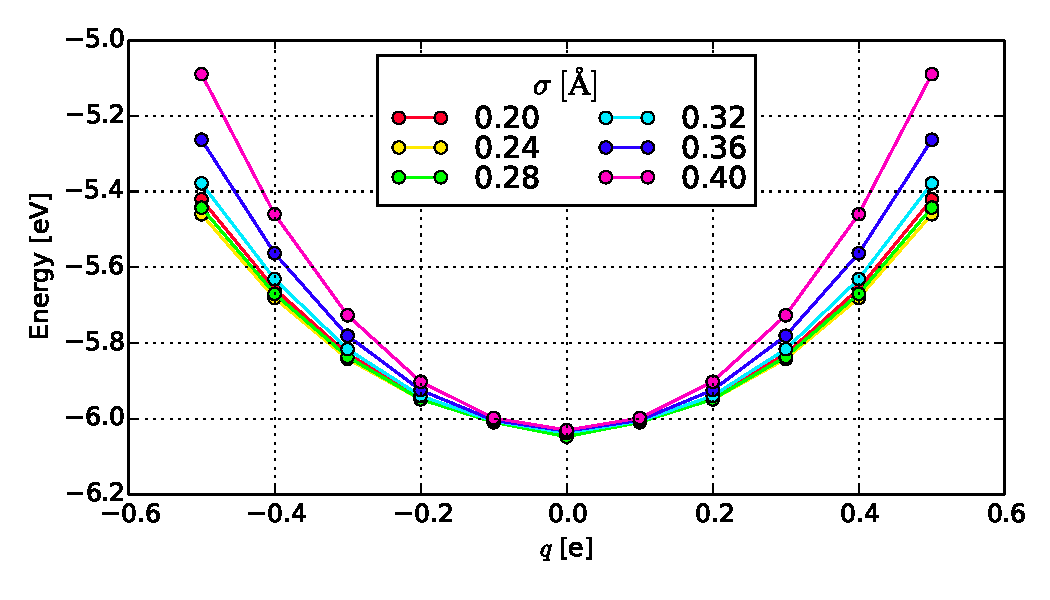
\includegraphics[width = 10cm]{Images/Hydrogen/charging/gaussian_sigmas}
	\caption{Ground state energy in respect to the displaced charge for different standard deviations $\sigma$ of the \textsc{Gaussian} curves.}
	\label{image_gaussian_sigmas_hydrogen}
\end{figure}
In the next step an appropriate modification of the tight binding model is needed to describe this charge displacements. The simplest approach would be to assume that all states $\Psi_k^{(v)}$ contribute equally to the charge displacement and that the general form of the new eigenstates can be approximated as:
\begin{align}
\Psi_k^{(v)}(q) &= \sqrt{\frac{1}{2}-\frac{q}{2}}c_k^{\dagger(e)}- \sqrt{\frac{1}{2}+\frac{q}{2}}\frac{\epsilon_k - i \Delta_k}{|E_k|}c_{k}^{\dagger(o)}
\end{align}
where $q$ denotes the displaced charge. These states show the needed behavior:
\begin{align}
	2\sum_k\left\langle\Psi_k^{(v)}(q)\Big|\hat{n}_k^{(e/o)}\Big|\Psi_k^{(v)}(q)\right\rangle &= N \left(1 \pm q\right)
\end{align}
which corresponds with a charge transfer of $q$ in each unit cell. Further these states have an energy expectation value of:
\begin{align}
\left\langle\Psi_k^{(v)}(q)\Big|\mathcal{H}_{k}\Big|\Psi_k^{(v)}(q)\right\rangle &= -\sqrt{1-q^2} |E_k|
\end{align}
Finally the assumption that the ground state energy can be approximated by the sum of the single electron energies is made, what leads to the expression:
\begin{align}
E_0(q) &= -\frac{4Nt_0}{\pi} \sqrt{1-q^2}
\label{equation_ground_state_energy_charge}
\end{align}
Many assumptions are made up to this point, that have to be tested. But before doing this, some issue with the quantity $q$ is discussed.\\
\begin{figure}
	\centering
	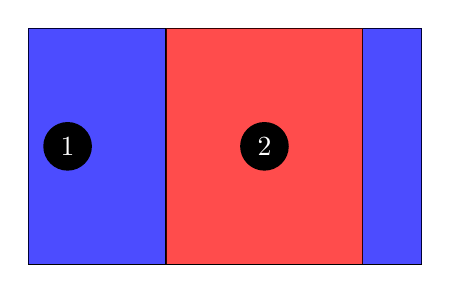
\begin{tikzpicture}
	\begin{scope}
	\clip [draw] (-.5, -1.5) rectangle (4.5, 1.5);
	\draw [fill = blue, opacity = 0.7] (-0.5, -1.5) rectangle (4.5, 1.5);
	\draw [fill = white, opacity = 1] (1.25, -1.5) rectangle (3.75, 1.5);
	\draw [fill = red, opacity = 0.7] (1.25, -1.5) rectangle (3.75, 1.5);
	\foreach \x/\num in {0/1, 2.5/2}{
		\node[fill = black, shape = circle, text = white] at (\x, 0)	 {\num};}
	\end{scope}
	\end{tikzpicture}
	\caption{Scheme: Integration regions (\textcolor{red}{red} and \textcolor{blue}{blue}) to calculate a 'tight binding charge' $q$.}
	\label{image_tight_binding_q_regions}
\end{figure}
\begin{figure}
	\centering
	\begin{subfigure}{0.49\textwidth}
		\centering
		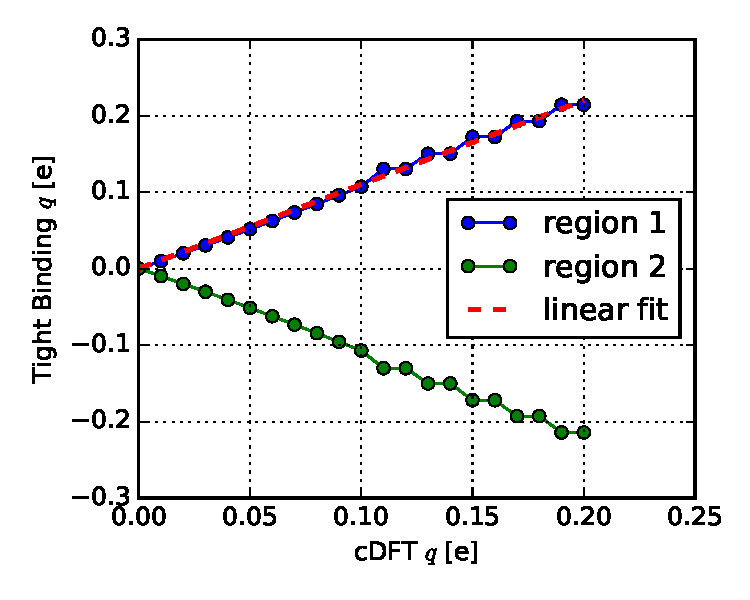
\includegraphics[width = \textwidth]{Images/Hydrogen/charging/qs_normal_sigma}
		\caption{$\sigma = \unit[0.24]{\AA}$}
		\label{}
	\end{subfigure}\hspace*{.5cm}
	\begin{subfigure}{0.49\textwidth}
		\centering
		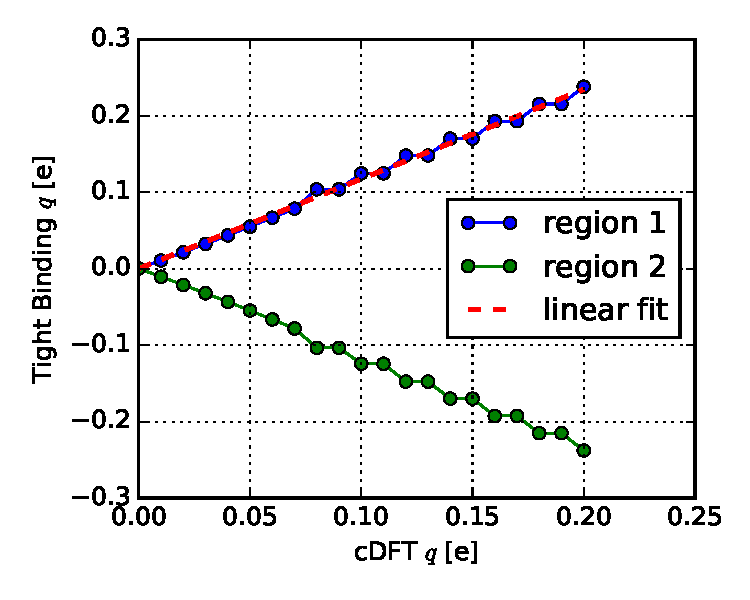
\includegraphics[width = \textwidth]{Images/Hydrogen/charging/qs_other_sigma}
		\caption{$\sigma = \unit[0.32]{\AA}$}
		\label{}
	\end{subfigure}
	\caption{Tight binding $q$ in respect to the cDFT q with a linear fit for different $\sigma$.}
	\label{image_qs_hydrogen}
\end{figure}
From the tight binding point of view $q$ denotes the charge belonging to some distinct core. On the other hand there is the $q$ appearing in the cDFT code, describing the integral over the charge density weighted with some \textsc{Gaussian} curves centered at the core positions. Even if they look somehow similar, they can't be simply assumed to be the same. To get some relation between them a 'tight binding' $q$ has to be calculated out of the charge density. Here the most natural approach seems to associate the charge at any point with the nearest core. This can be done by dividing the unit cell into separate parts and integrating the charge density over each such region (see \cref{image_tight_binding_q_regions}).\\
In \cref{image_qs_hydrogen} a linear dependency between the tight binding and cDFT charge can be seen, from which a proportionality constant can be calculated. For $\sigma = \unit[0.24]{\AA}$ the relation $q_\text{tb} \approx 1.10\cdot q_\text{cDFT}$ and for $\sigma = \unit[0.32]{\AA}$ the relation $q_\text{tb} \approx 1.17\cdot q_\text{cDFT}$ is obtained.\\
Using these proportionality constants $c$ the ground state energy can be fitted to the following expression\footnote{$N=2$, because the unit cell contains two hydrogen atoms.} (compare \cref{equation_ground_state_energy_charge}):
\begin{align}
	E_0(q) &= -\frac{8t_0}{\pi} \sqrt{1 - \left(c\cdot q_\text{cDFT}\right)^2}
\end{align}
\begin{figure}
	\centering
	\begin{subfigure}{0.49\textwidth}
		\centering
		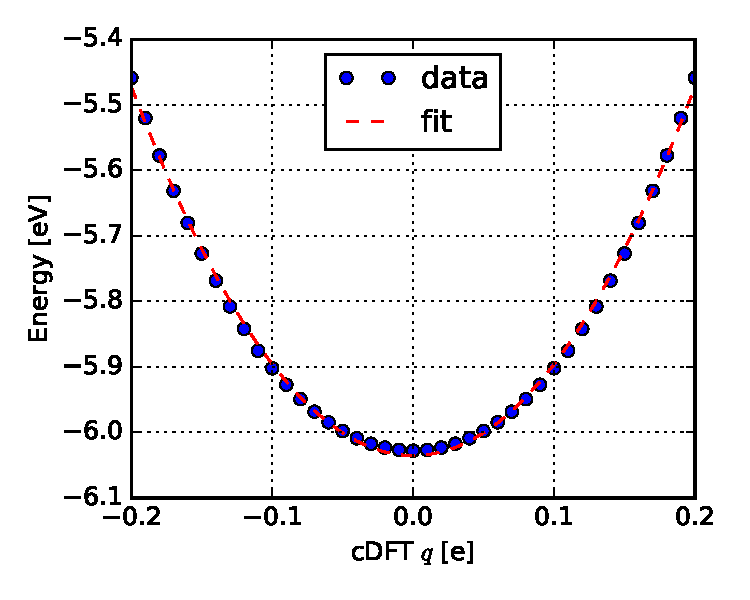
\includegraphics[width = \textwidth]{Images/Hydrogen/charging/energy_fit_normal_sigma}
		\caption{$\sigma = \unit[0.24]{\AA}$}
		\label{}
	\end{subfigure}\hspace*{.5cm}
	\begin{subfigure}{0.49\textwidth}
		\centering
		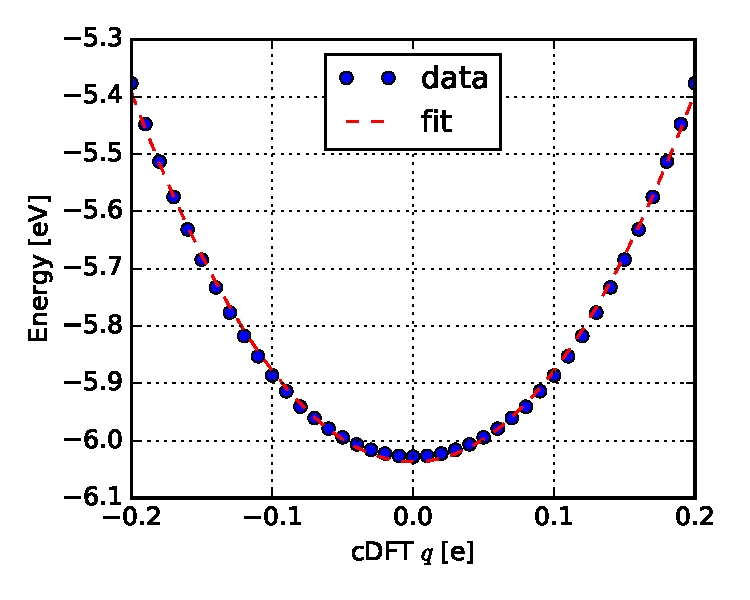
\includegraphics[width = \textwidth]{Images/Hydrogen/charging/energy_fit_other_sigma}
		\caption{$\sigma = \unit[0.32]{\AA}$}
		\label{}
	\end{subfigure}
	\caption{Ground state energy in respect to the displaced charge for different $\sigma$.}
	\label{image_ground_state_hydrogen_qs}
\end{figure}
As can be seen in \cref{image_ground_state_hydrogen_qs} the fits match the data for both $\sigma$ well. The so obtained hopping parameters are:
\begin{compactitem}
	\item $t_0 = \unit[9.0]{eV}$ for $\sigma = \unit[0.24]{\AA}$ and the corresponding proportionality constant $c = 1.10$
	\item $t_0 = \unit[9.1]{eV}$ for $\sigma = \unit[0.32]{\AA}$ and the corresponding proportionality constant $c = 1.17$
	\item $t_0 = \unit[10.3]{eV}$ for $\sigma = \unit[0.32]{\AA}$ and the proportionality constant $c = 1.10$ (just for comparison)
\end{compactitem}
Two things can be seen from this. First, the hopping parameters do not match the earlier calculated value of $t_0 = \unit[4.8]{eV}$ and thus there must have been some wrong assumptions in the derivation. Second, the values for different $\sigma$ are in good agreement if the correct proportionality constants are used. (Two other values are tested right now!)\\
A second approach to modify the tight binding model for cDFT is the following:\\
Modify the hopping Hamiltonian to decrease/increase the energies at the even/odd positions (matrix notation):
\begin{align}
\begin{pmatrix*}[c]
0 & \epsilon_k + i \Delta_k \\
\epsilon_k - i \Delta_k & 0
\end{pmatrix*} 
&\to 
\begin{pmatrix*}[c]
-V & \epsilon_k + i \Delta_k \\
\epsilon_k - i \Delta_k & V
\end{pmatrix*}
\end{align}
with the eigenenergies $E_k = \pm \sqrt{V^2+\epsilon_k^2+\Delta_k^2}$ and the eigenstates\footnote{the valence state corresponds with the lower signs} (vector notation):
\begin{align}
\vv{\Psi}_k(V) &= \frac{1}{\sqrt{2\left(E_k^2\mp V|E_k|\right)}}\cdot \begin{pmatrix*}[c]
-V\pm \sqrt{V^2+\epsilon_k^2+\Delta_k^2}\\
\epsilon_k - i \Delta_k
\end{pmatrix*}
\end{align}
For $V=0$ this matches the previous result. The sum over the HOMO-band energies becomes approximately:
\begin{align}
	E_0 &= \frac{-2N}{\pi} \sqrt{V^2+4t_0^2}
	\label{equation_ext_pot}
\end{align} 
Next, the band structure for the hydrogen chain with different charge displacements is calculated (see \cref{image_hydrogen_charged_bands}). As expected from the symmetry, the form of the band structures do not depend on the direction (sign) of the charge displacement. It can also be seen, that the influence of charging is bigger for $k$-points closer to the edge of the \textsc{Brillouin} zone and the bands are shifted to lower energies. Both is in good agreement with the predictions of the second approach.

\begin{figure}
	\centering
	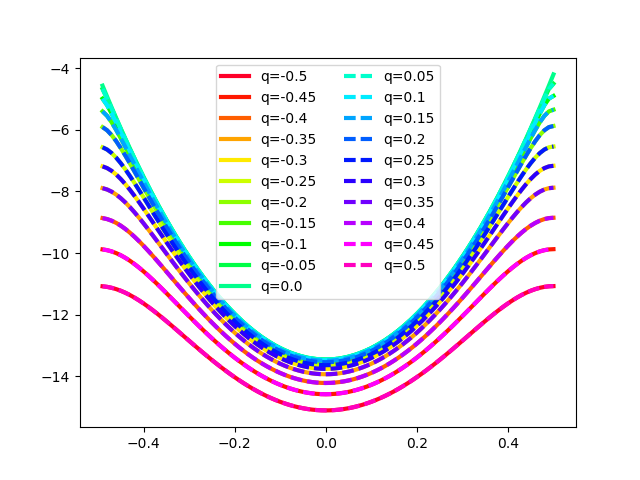
\includegraphics[width = 12cm]{Images/Hydrogen/hydrogen_charged_bands}
	\caption{Band structure of the HOMO-band for different charge displacements.}
	\label{image_hydrogen_charged_bands}
\end{figure}




In \cref{image_hydrogen_charge_potential} the height of the Gaussian potentials causing the charge displacement as a function of the transferred charge is shown. Again the symmetry is as expected and in the region of $-0.2 \le q \le 0.2$ the dependency is approximately linear.

\begin{figure}
	\centering
	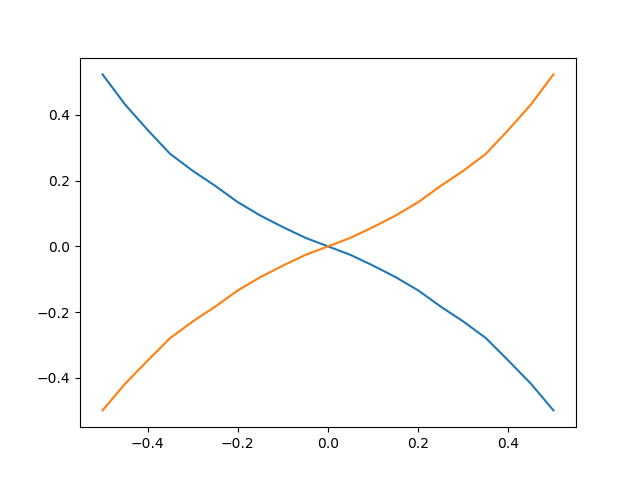
\includegraphics[width = 10cm]{Images/Hydrogen/hydrogen_charge_potential}
	\caption{$V(q)$}
	\label{image_hydrogen_charge_potential}
\end{figure}

From the model Hamiltonian the state energy at the edge of the Brillouin zone ($k\cdot a = \nicefrac{\pi}{2}$) is expected to have the form $E_\text{edge} = -\sqrt{V^2} = -\sqrt{c^2\cdot U_\text{CDFT}^2}$. As can be seen in \cref{image_hydrogen_border_energy_potential} this matches the results of the simulation very well. From a fit to this data the ratio between the theoretical potential and the voltage from CDFT can be obtained: $V \approx \unit[13.265]{e} \cdot U_\text{CDFT}$.

\begin{figure}
	\centering
	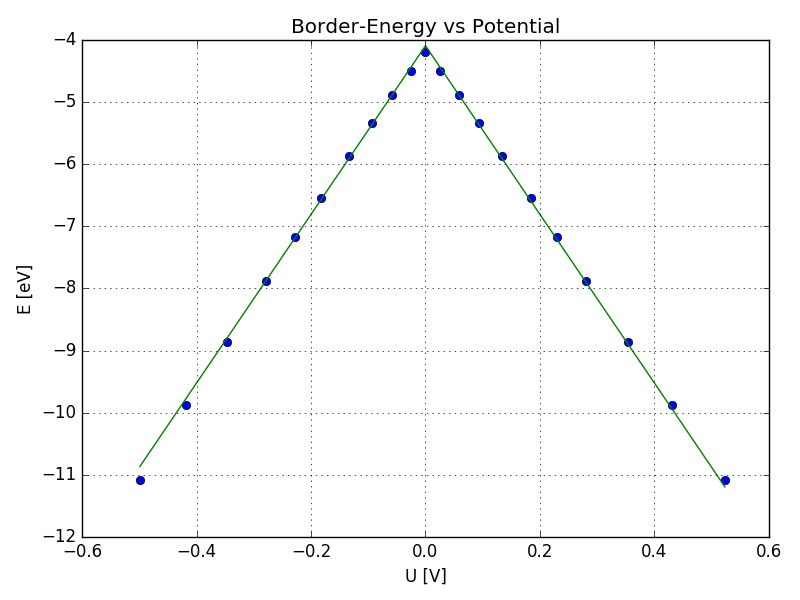
\includegraphics[width = 12cm]{Images/Hydrogen/hydrogen_border_energy}
	\caption{$E(U)$}
	\label{image_hydrogen_border_energy_potential}
\end{figure}

Analogously this ratio can be calculated by fitting the energy at the gamma point to \linebreak $E_\text{gamma} = -\sqrt{c^2 \cdot U_\text{CDFT}^2 + 4 \cdot t_0^2}$ (see \cref{image_hydrogen_mid_energy_potential}). Here the proportionality constant becomes $V \approx \unit[11.289]{e} \cdot U_\text{CDFT}$, which corresponds to a relative difference of approximately 20\%. To take a closer look at this effect the proportionality constant is calculated by fitting for many different $k$-points (see \cref{image_hydrogen_proportionality_constant}). 
\begin{figure}
	\centering
	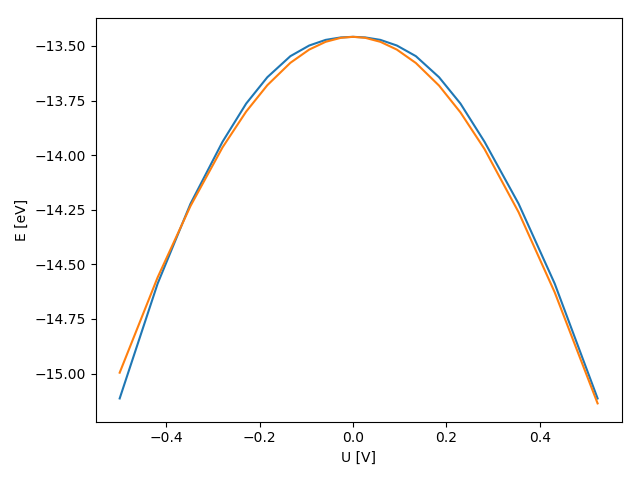
\includegraphics[width = 12cm]{Images/Hydrogen/hydrogen_mid_energy}
	\caption{$E(U)$}
	\label{image_hydrogen_mid_energy_potential}
\end{figure}

\begin{figure}
	\centering
	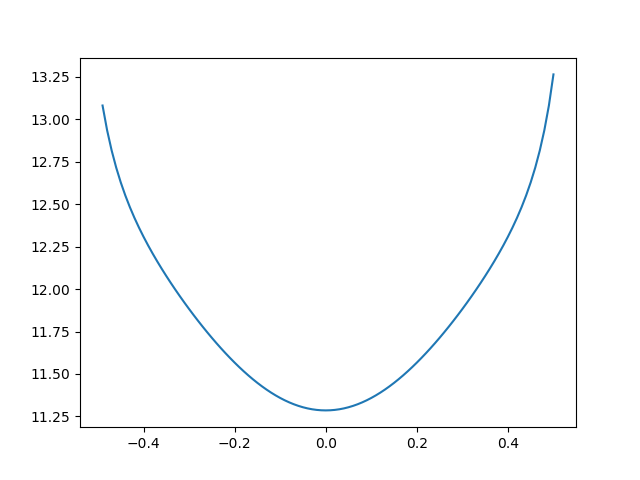
\includegraphics[width = 12cm]{Images/Hydrogen/hydrogen_c_k_dependency}
	\caption{$c(k)$}
	\label{image_hydrogen_proportionality_constant}
\end{figure}
For example the \textsc{Coulomb} repulsion of the electrons would be added twice and other terms of the exchange correlation energy would be left out.
\chapter{Things to do}
\begin{compactitem}
	\item Correlation check, charge regions
	\item Abstract
	\item Summary
	\item Appendix
	\item Uniform axis labels
\end{compactitem}